% Main file: compile with pdfLaTeX (or latexmk -pdf main.tex).
% TUM Thesis for Informatics layout from the linked Overleaf template.
\documentclass[headsepline,footsepline,footinclude=false,oneside,fontsize=11pt,paper=a4,listof=totoc,bibliography=totoc,DIV=12]{scrbook}
% Adapted from fwalch/tum-thesis-latex, the upstream named by the linked
% Overleaf template (Tobias Weiher, 2018). See TEMPLATE_LICENSE.md.
\PassOptionsToPackage{table,svgnames,dvipsnames}{xcolor}
\usepackage[utf8]{inputenc}
\usepackage[T1]{fontenc}
\usepackage{lmodern}
\usepackage[sc]{mathpazo}
\IfFileExists{ngerman.ldf}{\usepackage[ngerman,english]{babel}}{\usepackage[english]{babel}\babelprovide[import]{ngerman}}
\usepackage{amsmath,amssymb}
\usepackage[authoryear,round]{natbib}
\usepackage{xcolor}
\usepackage{graphicx}
\usepackage{booktabs,array,longtable}
\usepackage[final]{microtype}
\usepackage{caption}
\usepackage{fvextra}
\usepackage{upquote}
\usepackage[hyphens]{url}
\usepackage{xurl}
\usepackage[hidelinks,breaklinks]{hyperref}
\usepackage{placeins}
\setkomafont{disposition}{\normalfont\bfseries}
\linespread{1.05}
\setlength{\emergencystretch}{2em}
\setlength{\LTleft}{0pt plus 1fill}
\setlength{\LTright}{0pt plus 1fill}
\captionsetup{font=small,labelfont=bf,singlelinecheck=false}
\BeforeTOCHead[toc]{{\cleardoublepage\pdfbookmark[0]{\contentsname}{toc}}}
\definecolor{TUMBlue}{HTML}{0065BD}
\definecolor{TUMSecondaryBlue}{HTML}{005293}
\definecolor{TUMSecondaryBlue2}{HTML}{003359}
\definecolor{TUMBlack}{HTML}{000000}
\definecolor{TUMWhite}{HTML}{FFFFFF}
\definecolor{TUMDarkGray}{HTML}{333333}
\definecolor{TUMGray}{HTML}{808080}
\definecolor{TUMLightGray}{HTML}{CCCCC6}
\definecolor{TUMAccentGray}{HTML}{DAD7CB}
\definecolor{TUMAccentOrange}{HTML}{E37222}
\definecolor{TUMAccentGreen}{HTML}{A2AD00}
\definecolor{TUMAccentLightBlue}{HTML}{98C6EA}
\definecolor{TUMAccentBlue}{HTML}{64A0C8}
\addto\captionsenglish{\renewcommand{\bibname}{References}}
\DeclareTOCStyleEntry[numwidth=3em]{tocline}{table}
\DeclareTOCStyleEntry[numwidth=3em]{tocline}{figure}
\setlength{\bibsep}{0.65\baselineskip}

% Edit only these fields to complete the template's title pages.
\newcommand*{\getUniversity}{Technische Universität München}
\newcommand*{\getFaculty}{Department of Informatics}
\newcommand*{\getTitle}{Graph-Aware Prompting for Entity Typing}
\newcommand*{\getSubtitle}{Leveraging Taxonomy Structure in Large Language Models}
\newcommand*{\getTitleGer}{[German title to be confirmed]}
\newcommand*{\getAuthor}{Sindi Teqja}
\newcommand*{\getDoctype}{Bachelor's Thesis}
\newcommand*{\getSupervisor}{[Supervisor name]}
\newcommand*{\getAdvisor}{[Advisor name]}
\newcommand*{\getSubmissionDate}{15 October 2026}
\newcommand*{\getSubmissionLocation}{[Place of signing]}

\hypersetup{pdftitle={Graph-Aware Prompting for Entity Typing},pdfauthor={Sindi Teqja}}
\begin{document}
\selectlanguage{english}
\pagenumbering{alph}
\begin{titlepage}
  % HACK for two-sided documents: ignore binding correction for cover page.
  % Adapted from Markus Kohm's KOMA-Script titlepage=firstiscover handling.
  % See http://mirrors.ctan.org/macros/latex/contrib/koma-script/scrkernel-title.dtx,
  % \maketitle macro.
  \oddsidemargin=\evensidemargin\relax
  \textwidth=\dimexpr\paperwidth-2\evensidemargin-2in\relax
  \hsize=\textwidth\relax

  \centering

  \IfFileExists{logos/tum.pdf}{%
    
\includegraphics[height=20mm]{logos/tum.pdf}
  }{%
    \vspace*{20mm}
  }

  \vspace{5mm}
  {\huge\MakeUppercase{\getFaculty{}}}\\

  \vspace{5mm}
  {\large\MakeUppercase{\getUniversity{}}}\\

  \vspace{20mm}
  {\Large \getDoctype{}}

  \vspace{15mm}
  {\huge\bfseries \getTitle{}\par\vspace{4mm}{\Large\normalfont \getSubtitle{}}}

  \vspace{15mm}
  {\LARGE \getAuthor{}}

  \IfFileExists{logos/faculty.pdf}{%
    \vfill{}
    
\includegraphics[height=20mm]{logos/faculty.pdf}
  }{}
\end{titlepage}

\frontmatter
\begin{titlepage}
  \centering

  \IfFileExists{logos/tum.pdf}{%
    
\includegraphics[height=20mm]{logos/tum.pdf}
  }{%
    \vspace*{20mm}
  }

  \vspace{5mm}
  {\huge\MakeUppercase{\getFaculty{}}}\\

  \vspace{5mm}
  {\large\MakeUppercase{\getUniversity{}}}\\

  \vspace{20mm}
  {\Large \getDoctype{}}

  \vspace{15mm}
  {\huge\bfseries \getTitle{}\par\vspace{4mm}{\Large\normalfont \getSubtitle{}} \par}

  \vspace{10mm}
  {\huge\bfseries \foreignlanguage{ngerman}{\getTitleGer{}} \par}

  \vspace{15mm}
  \begin{tabular}{l l}
    Author:          & \getAuthor{} \\
    Supervisor:      & \getSupervisor{} \\
    Advisor:         & \getAdvisor{} \\
    Submission Date: & \getSubmissionDate{} \\
  \end{tabular}

  \IfFileExists{logos/faculty.pdf}{%
    \vfill{}
    
\includegraphics[height=20mm]{logos/faculty.pdf}
  }{}
\end{titlepage}

\thispagestyle{empty}
\vspace*{0.8\textheight}
\noindent
I confirm that this \MakeLowercase{\getDoctype{}} is my own work and I have documented all sources and material used.

\vspace{15mm}
\noindent
\getSubmissionLocation{}, \getSubmissionDate{} \hspace{50mm} \getAuthor{}

\cleardoublepage{}

\addchap{Abstract}

Entity typing assigns semantic categories to entities. When categories form a taxonomy, a useful prediction must identify a suitable specific type, recover relevant broader types, and distinguish nearby alternatives. This thesis investigates whether presenting local taxonomy structure together with instructions for interpreting it improves that task for large language models. The central comparison holds the entity, description, and prompting style fixed while changing both structural evidence and graph-specific instructions. Three styles are examined: standard prompting, chain-of-thought prompting, and contrastive chain-of-thought prompting.


The study uses the released 1,000-entity WiKC evaluation sample and the refined Wikidata taxonomy introduced by Peng, Bonald, and Alam (2024). Nine conditions are evaluated with Gemini 3.8 Flash and Llama 3.1 8B Instruct; Llama is run with seeds 0, 42, and 123. The supplied archives contain 9,000 completed Gemini responses and 8,991, 8,971, and 8,986 completed main Llama responses, respectively. A further child-removal experiment at Llama seed 0 completes 1,352 of 1,353 planned responses for 451 eligible entities. Within-model contrasts use matched successful responses. Context is selected around an annotated gold class, whose label is omitted; the experiment therefore measures the value of oracle structural evidence rather than autonomous retrieval.


Graph-aware prompting improves mean entity F1 in every model-by-style comparison, with paired gains from 0.0451 to 0.1348. Parent-only context outperforms sibling-only context on aggregate F1. The three Llama seeds permit a direct check of sampling variation, while the matched child intervention separates child-context effects from differences in cohort composition. The results are interpreted together with output length, ranking metrics, and condition-specific completion rates.


The empty-child control gives small positive point estimates (about +0.005 to +0.024); Gemini’s roughly +0.02 contrasts with its +0.0625 standard graph gain. This suggests a template contribution, but different cohorts prevent attributing a fixed share of the full gain to instructions.


These findings support graph-aware prompting as a useful source of evidence under controlled context selection. The contribution is a reproducible prompting and evaluation framework, together with an empirical account of where local structure helps and where it misleads. Future work should evaluate retrieved context, independently annotated gold sets, and controlled structural noise.


{\small Keywords: entity typing, knowledge graphs, taxonomy, prompting, WiKC, evaluation\par}


\microtypesetup{protrusion=false}
{\small\tableofcontents}
\microtypesetup{protrusion=true}
\addchap{Reading conventions}

“Graph” denotes supplied local WiKC taxonomy context and its interpretation instructions. “No graph” denotes the entity and description without that context. “Gemini” denotes gemini-3.8-flash through the Gemini API \citep{googledeepmind2026}; “Llama” denotes the fixed Llama 3.1 8B Instruct checkpoint described in Section 5.4. Standard, CoT, and contrastive name the three prompt styles.


Unless stated otherwise, condition means use completed responses; paired differences use the intersection of completed responses, with n reported. F1 is the arithmetic mean of entity-level F1 scores. Differences are graph minus no graph, or children included minus children removed. Figures print four decimals. Bootstrap intervals describe entity variation; Llama seed variation is reported separately.


\mainmatter
\chapter{Introduction}

\FloatBarrier

\section{Structural evidence in entity typing}

Knowledge graphs provide a representation in which entities and categories can be connected through explicit relations. Their schema and identity conventions determine what those connections mean \citep{hogan2021}. A taxonomy is particularly relevant here because its subclass relations specify which categories are broader or narrower. WiKC provides a refined taxonomy and an evaluation resource derived from Wikidata \citep{peng2024}. It makes the experimental context auditable: the researcher can inspect the supplied neighbours and the annotated hierarchy associated with each entity.


A framboid is described in the evaluation data as a “minute spheroidal grain of pyrite or an aggregate of such grains”, with further geological context. Its selected gold centre is crystal, a label absent from that description. The supplied parent chemical substance and nearby sibling classes provide a structural frame for identifying the intended category and its broader types. A typing system must decide which categories the description supports and how to order them. If it produces a nearby category instead, its answer may sound reasonable while failing to recover the intended class.


This thesis studies that problem through graph-aware prompting. A prompt supplies local relations around an omitted centre class: its parents, its siblings, and its children. Parents indicate a broader semantic scope. Siblings expose nearby alternatives. Children illustrate distinctions that require additional evidence. The model must combine this structure with the entity description, rather than copy all neighbours into its output. The research question concerns the effect of these structural relations on predictions, not merely whether one model achieves a larger aggregate score.


The empirical outcome is encouraging but conditional. Graph-aware prompting improves F1 in all model-by-style comparisons, including each Llama seed. However, the context is selected using the annotated answer. This gives the model privileged structural information even though the centre label itself is hidden. The experiment consequently asks how much a model gains when relevant local structure and its interpretation instructions are available.


\FloatBarrier

\section{Contributions}

C1. A fixed one-shot prompt design for ranked entity typing, with three styles and parent-, sibling-, and child-context conditions.


C2. Matched comparisons of two model systems, three Llama seeds, and a child-removal intervention at Llama seed 0.


C3. An evaluation separating label-set recovery, maximum-depth type recovery, and ordering, with explicit failure counts and auditable prompt and response records.


\FloatBarrier

\section{Research questions and hypotheses}

RQ1. Does graph-aware prompting improve entity typing when the model, entity, description, and prompting style are fixed?


RQ2. How do parent, sibling, and child conditions contribute, and does removing children change predictions for entities with child context?


RQ3. How do graph gains vary with maximum annotated taxonomy depth?


RQ4. How do the evaluated Gemini and Llama systems differ in performance and response to graph context?


RQ1 is primary and concerns the combined change in evidence and instructions. Its design consists of three paired contrasts per model and Llama seed. RQ4 is a supporting comparison of concrete systems because deployment, model size, decoding, and implementation differ. RQ2 includes a child-removal comparison restricted to the 451 eligible entities.


H1. Sibling-only context is the most useful individual relation condition for entity F1. H2. The benefit of graph-aware prompting increases with maximum gold depth. These hypotheses are evaluated explicitly in Sections 7.4 and 7.6; they are not revised after observing the results.


The study is exploratory. Entities used during prompt development remain in the final cohort. Each completed condition yields one accepted response per entity and seed after format recovery where needed; Llama is evaluated with three seeds. There is no sealed test set. Entity bootstrap intervals and between-seed variation quantify different sources of uncertainty.


\FloatBarrier

\section{Thesis outline}

Chapter 2 defines the task and notation. Chapter 3 positions the work in the literature. Chapters 4–6 describe the data, method, and evaluation. Chapter 7 answers RQ1–RQ4, and Chapter 8 discusses the findings. Chapter 9 concludes; Chapter 10 presents limitations and future research. The appendices provide full scores, reproducibility details, and the nine complete prompts.


\chapter{Preliminary concepts}

\FloatBarrier

\section{Taxonomy and local relations}

The definitions below fix the notation used in Chapters 4–6. Graph terminology follows the distinctions between identifiers, labels, and relations discussed by \citet{hogan2021}. Hierarchy closure follows the evaluation framework discussed by \citet{kosmopoulos2015} and \citet{plaud2024}.


{\small \textbf{Definition 2.1 (Taxonomy).} A taxonomy is T = (C, E, r, \ensuremath{\lambda}), where C is a finite set of class identifiers, E \ensuremath{\subseteq} C \ensuremath{\times} C is an acyclic subclass relation, r is the root, and \ensuremath{\lambda} maps class identifiers to readable labels. An edge (c, p) points from child c to immediate parent p. The root is entity (wd:Q35120). Labels need not uniquely identify classes. A knowledge graph more generally represents entities and relations; T is its class-hierarchy component.\par}


{\small \textbf{Definition 2.2 (Relations and closure).} For c \ensuremath{\in} C, Par(c) = \{p : (c,p) \ensuremath{\in} E\}, Ch(c) = \{x : (x,c) \ensuremath{\in} E\}, and Sib(c) = (\ensuremath{\cup}\textsubscript{p\ensuremath{\in}Par(c)} Ch(p)) \ensuremath{-} \{c\}. Anc(c) contains nodes reachable from c by a nonempty upward path; Desc(c) contains nodes with a nonempty path to c. For a class set A, U(A) = A \ensuremath{\cup} \ensuremath{\cup}\textsubscript{c\ensuremath{\in}A} Anc(c) is its upward closure, including roots. A is ancestor-closed exactly when U(A) = A. Siblings share a parent and need not be disjoint.\par}


{\small \textbf{Definition 2.3 (Depth).} The depth d(c) is the shortest-path length from c to r following child-to-parent edges, equivalently from r to c in the reversed graph. In a multiple-inheritance DAG it may differ from the longest path length. The evaluation uses the released annotated depths. A label recorded in the annotations but absent from the edge graph retains its supplied depth and has no traversable neighbours in this implementation.\par}


\FloatBarrier

\section{Entities, gold annotations, and centre selection}

{\small \textbf{Definition 2.4 (Entity and gold sets).} An entity e = (id(e), n(e), \ensuremath{\delta}(e)) has an identifier, name, and description. The evaluation set is D, with |D| = 1,000. G(e) is the set of class identifiers listed for e in the released evaluation file, with their labels and annotated depths; it is not replaced by U(G(e)) for flat scoring. The graph-minimal gold set is G\textsubscript{min}(e) = \{c \ensuremath{\in} G(e) : Desc(c) \ensuremath{\cap} G(e) = \{\}\}. Define d\textsubscript{max}(e) = max\textsubscript{c\ensuremath{\in}G(e)} d(c) and G\textsubscript{max}(e) = \{c \ensuremath{\in} G(e) : d(c) = d\textsubscript{max}(e)\}. Graph minimality and maximum shortest-path depth are distinct properties.\par}


{\small \textbf{Definition 2.5 (Centre).} The centre c*(e) is the member of G\textsubscript{min}(e) with greatest annotated depth, breaking ties by ascending lexicographic order of the class-identifier strings (for example, the full wd:Q… string), not numerical Q-ID order. If that candidate set is empty, the implementation applies the same ordering to G(e). The centre label is \ensuremath{\lambda}(c*(e)). Context uses this one centre; MRR evaluates the set G\textsubscript{max}(e). These objects need not coincide in a DAG.\par}


\FloatBarrier

\section{Context and ranked entity typing}

{\small \textbf{Definition 2.6 (Local context).} For relation R \ensuremath{\in} \{Par, Sib, Ch\}, L\textsubscript{R,k}(c) is the first k identifiers in R(c) sorted lexicographically, with k = 3. For a chosen relation set A, the local context K\textsubscript{A,k}(c) consists of these labelled relation lists. The centre itself is excluded from the lists; unavailable lists are empty. A centre absent from the edge graph receives empty lists. Context is oracle-selected when c = c*(e) is computed from gold annotations.\par}


{\small \textbf{Definition 2.7 (Ranked entity typing).} Given n(e), \ensuremath{\delta}(e), a prompting condition, and optionally K\textsubscript{A,3}(c*(e)), the model returns an ordered finite list P(e) = (p\textsubscript{1}, …, p\textsubscript{m}) of type-label strings, intended to run from specific supported types to broader valid types. Explanation-bearing conditions also return text, but this text is not itself scored as a type. Gold classes determine evaluation and oracle selection; the complete gold list is not presented as the test entity’s answer.\par}


{\small \textbf{Definition 2.8 (Normalization, matching, and resolution).} N(s) case-folds a string, replaces underscores with spaces, collapses whitespace, and strips surrounding whitespace and the punctuation . , ; : ! ? and quotation marks. A prediction matches a gold label exactly when their normalized strings are equal; no semantic aliases are added. Let L(q) be the identifiers whose supplied labels normalize to q. Resolution maps an exact gold-label match to all matching annotated class identifiers; otherwise it maps q only when |L(q)| = 1. An unresolved prediction remains an opaque false-positive item in hierarchical precision.\par}


{\small \textbf{Definition 2.9 (Prompting condition).} A condition is (s,A), with style s \ensuremath{\in} \{standard, CoT, contrastive\} and relation set A \ensuremath{\subseteq} \{Par,Sib,Ch\}. The main design uses A = \{\} and A = \{Par,Sib,Ch\} for each style, plus the three singleton relation sets for standard prompting. Each condition contains its own frozen instructions and one external demonstration. Thus graph-versus-no-graph compares a package of evidence and interpretation instructions, not evidence alone.\par}


\FloatBarrier

\section{Evaluation quantities}

{\small \textbf{Definition 2.10 (Set recovery).} Let \ensuremath{\hat{P}}(e) be the set of unique normalized predictions and \ensuremath{\hat{G}}(e) = \{N(\ensuremath{\lambda}(c)) : c \ensuremath{\in} G(e)\}. Precision is |\ensuremath{\hat{P}} \ensuremath{\cap} \ensuremath{\hat{G}}| / |\ensuremath{\hat{P}}|, recall is |\ensuremath{\hat{P}} \ensuremath{\cap} \ensuremath{\hat{G}}| / |\ensuremath{\hat{G}}|, and entity F1 is 2|\ensuremath{\hat{P}} \ensuremath{\cap} \ensuremath{\hat{G}}| / (|\ensuremath{\hat{P}}| + |\ensuremath{\hat{G}}|), with zero for an empty predicted set. Reported macro F1 is the arithmetic mean of entity F1. Hierarchical F1 applies the same set formula after resolving labels and expanding both sides with U, retaining unresolved predictions as separate items.\par}


{\small \textbf{Definition 2.11 (Ranking).} Reciprocal rank is 1/j for the first rank j matching any label in G\textsubscript{max}(e), and zero if none matches. MRR averages this value. For nDCG, a gold label has relevance equal to its largest annotated depth divided by d\textsubscript{max}(e); unmatched labels and repeated credited labels have relevance zero. DCG = \ensuremath{\Sigma}\textsubscript{j=1…K} (2\textsuperscript{rel\textsubscript{j}} \ensuremath{-} 1)/log\textsubscript{2}(j+1), and nDCG = DCG/IDCG, where IDCG sorts all gold relevances decreasingly and K is the larger of prediction length, unique gold-label count, and one. If all gold depths are zero, gold relevance is one. This is the project’s depth-weighted application of Järvelin and Kekäläinen’s (2002) framework.\par}


\chapter{Related work and motivation}

\FloatBarrier

\section{Structured evidence for language models}

The integration of language models and knowledge graphs includes several distinct directions. \citet{pan2024} organize work on using graphs to support language models, using language models to support graph construction, and combining the two in broader systems.


StructGPT uses interfaces to access structured data and an iterative reading-and-reasoning procedure \citep{jiang2023}. Think-on-Graph explores graph-guided reasoning with language models \citep{sun2024}. These systems motivate the use of relations as evidence, but their graph access and reasoning tasks differ from the fixed neighbourhoods used here. The present experiment does not perform autonomous multi-step traversal. It linearizes a small, preselected neighbourhood into a prompt and asks for an ordered label list.


This simpler design isolates a useful question. A sophisticated retrieval system can fail because it finds the wrong nodes, because it presents them poorly, or because the model misinterprets them. Oracle neighbourhoods remove much of the retrieval problem and make the interpretation stage visible. If correctly selected local relations did not improve typing, investing in retrieval would have a weaker empirical rationale. Because they do improve it, the next research step is to test how much of that benefit survives imperfect selection.


Relevant evidence is not necessarily harmless evidence. \citet{shi2023} demonstrated distraction from irrelevant information in arithmetic reasoning. \citet{liu2024} showed that the position of useful information in long contexts can affect performance. These results motivate concise neighbourhoods and careful context controls. They do not prove that the exact same failure mechanism operates in entity typing. The current study observes the effects of selected prompts; it does not independently manipulate context position or inject controlled noise in its final experiment.


The literature consequently supports both the structural hypothesis and the need for restraint. Explicit relations may anchor a semantic decision, but their selection, length, and interpretation remain empirical questions. The completed study addresses these questions through matched graph comparisons and relation ablations. It leaves dynamic traversal, retrieval precision, positional effects, and noisy graph robustness to subsequent work.


\FloatBarrier

\section{Taxonomy refinement and entity typing research}

WiKC is a refined Wikidata taxonomy constructed through a combination of graph operations and language-model judgments. \citet{peng2024} address redundant classes, problematic subclass links, and structural complexity. Their released resource provides both the graph and an entity-typing evaluation setting. This makes it suitable for examining whether already constructed local structure helps a different language model produce type labels.


Taxonomy enrichment asks a different question: how can additional valid classes or links be proposed and integrated? Ghamlouch and Alam’s (2025) Taxoria work uses an existing taxonomy as a seed and validates proposed additions. \citet{shen2025} combine sibling and parent generation in taxonomy-guided instruction tuning for expansion tasks. These approaches show that parent and sibling relations can support operations on a taxonomy, but they do not imply that sibling-only prompts will maximize entity-typing F1. The current results provide a separate downstream test.


Recent fine-grained typing research also emphasizes label semantics and candidate selection. \citet{ma2026} use entity and type descriptors in a retrieval-augmented framework that reduces the effective candidate space. This is relevant to the next stage of the project because a deployable graph-aware system must find suitable neighbourhoods from the entity description. The present oracle design supplies that neighbourhood directly and does not impose an explicit closed candidate list.


The distinction between fixed gold labels and semantic judgments matters when comparing evaluation approaches. WiKC’s original extrinsic evaluation examines type statements using a judge model. This thesis scores generated lists against the released annotations with a deterministic matching rule. Its numerical scores cannot therefore be compared directly with the original paper’s statement-validation accuracy. They answer different questions using different denominators and decision procedures.


The gap addressed here is a matched analysis of how local parent, sibling, and child evidence interacts with three prompting styles for ranked multi-label typing on the same WiKC cohort across two model systems.


\FloatBarrier

\section{Closely related typing approaches}

Wikidata provides the collaborative knowledge-base setting from which WiKC is derived \citep{vrandecic2014}. Hierarchy-aware mention typing predates current LLM prompting: \citet{xu2018} use hierarchy-aware loss to address noisy, overly specific labels; \citet{chen2020} combine multi-level ranking with coarse-to-fine decoding; \citet{onoe2021} use box embeddings to represent dependencies among fine-grained types. These approaches place structure in learned representations or supervised prediction, whereas the present study supplies a small neighbourhood as inference-time text.


For knowledge-graph entity typing, ConnectE connects entity and type embeddings using graph information \citep{zhao2020}, while TET encodes entity neighbours with a transformer \citep{hu2022}. These neighbours are evidence about an entity within a graph, rather than an oracle neighbourhood around its annotated type. OntoType uses ontology-guided prompting and natural-language inference for annotation-free fine-grained typing \citep{komarlu2024}. CASENT evaluates zero-and few-shot transfer and comparisons with large language models, showing why task-specific typing remains a relevant baseline \citep{feng2023}. These settings are related but their scores are not directly comparable with the present full-hierarchy exact-label evaluation.


LLM-based zero-and few-shot typing requires distinguishing demonstrations from supervised training. \citet{feng2023} evaluate ChatGPT with zero, eight, sixteen, and thirty-two demonstrations on ultra-fine typing: demonstrations improve coverage, but the open label inventory remains difficult. Their zero-shot tests on five smaller domain inventories instead provide all candidate labels. This shows why label-space constraints and demonstration count must be specified. Here the model receives one demonstration, generates an open label list, and is evaluated against a complete annotated hierarchy. \citet{ma2026} address a different constraint through descriptor-based candidate retrieval and LLM classification, with training-data filtering and fine-tuning. Their approach motivates a retrieved-context extension, whereas this thesis measures oracle-selected local relations without task-specific fine-tuning. Table~\ref{table:3.1} summarizes these distinctions.


\begingroup
\begin{table}[!htbp]
\setlength{\tabcolsep}{3pt}
\renewcommand{\arraystretch}{1.18}
\fontsize{8.5}{10.5}\selectfont
\renewcommand{\thetable}{3.1}
\caption{Positioning against closely related work.}\label{table:3.1}
\begin{tabular}{>{\raggedright\arraybackslash}p{\dimexpr 0.254902\linewidth-2\tabcolsep\relax}>{\raggedright\arraybackslash}p{\dimexpr 0.361656\linewidth-2\tabcolsep\relax}>{\raggedright\arraybackslash}p{\dimexpr 0.383442\linewidth-2\tabcolsep\relax}}
\toprule
\textbf{Work} & \textbf{Role of structure} & \textbf{Difference from this study} \\
\midrule
Xu \& Barbosa (2018) & Hierarchy-aware training loss & Supervised mention typing \\
Chen et al. (2020) & Sibling ranking and hierarchical decoding & Learned, constrained prediction \\
Onoe et al. (2021) & Type dependencies in box embeddings & Learned type representations \\
ConnectE (Zhao et al., 2020) & Entity/type graph embeddings & Graph-entity typing with learned embeddings \\
TET (Hu et al., 2022) & Transformer over entity neighbours & Graph-entity rather than class-centre context \\
OntoType (Komarlu et al., 2024) & Ontology-guided prompting and NLI & Coarse-to-fine candidate refinement \\
CASENT (Feng et al., 2023) & Calibrated type generation; zero/few-shot transfer & Trained seq2seq typing and LLM comparisons \\
DR-FET (Ma et al., 2026) & Descriptor-based candidate retrieval & Candidate-constrained LLM typing and fine-tuning \\
This thesis & Local class relations in one-shot prompts & Matched style/relation contrasts and ranked gold-chain recovery \\
\bottomrule
\end{tabular}
\end{table}
\endgroup


\chapter{Dataset and taxonomy}

\FloatBarrier

\section{Origin of the resource}

The data originate from the WiKC project of Peng, Bonald, and Alam (2024). The public repository identifies a Wikidata dump dated 22 March 2024 and provides the refined taxonomy, labels, and evaluation resources. The present thesis uses the released miniature evaluation file, wikc\_\allowbreak{}eval\_\allowbreak{}1k.txt, rather than collecting a new set of entities or manually creating an alternative taxonomy.


The original authors refine taxonomic links and merge redundant or equivalent classes using language-model semantic judgments together with graph processing. The released graph used by the project contains 16,581 class nodes and 19,622 directed links, consistent with the approximate 17,000 classes and 20,000 links described in the paper. The implementation checks that the loaded taxonomy is acyclic. Class identifiers and labels are stored separately, allowing traversal to use identifiers while prompts use readable labels.


The repository’s evaluation notebook explains the sample construction. It restricts eligible instances to those associated with English Wikipedia, maps source classes into WiKC or to surviving nearby ancestors, and reduces redundant type assignments. It constructs an instance pool with class-level sampling controls, then draws a 1,000-instance miniature sample. The exported file includes entity identifiers, labels, descriptions, class identifiers, and ancestor depths. These records are the basis of the current gold annotations (Peng et al., 2024; Peng et al., 2024, repository notebook).


One discrepancy requires explicit documentation. The paper describes a limit of 1,000 instances per class in its larger extrinsic evaluation. The inspected public notebook contains a comment with that value but executable code sampling 100 instances when a class exceeds 100. The thesis does not silently reconcile these statements or claim to have rerun the original sampling. It uses the released 1,000-entity file as the fixed experimental input. The archived file is authoritative for the present cohort, while the notebook provides the best available account of its construction.


The thesis author’s data construction occurs after this release. It groups repeated rows by entity, preserves all annotated classes and depths, selects a deterministic centre for context extraction, and generates nine prompt conditions per entity. These are derived experimental inputs, not new independent type judgments. Maintaining that distinction attributes the original dataset correctly and prevents the evaluation from implying a stronger annotation provenance than it has.


\FloatBarrier

\section{Cohort construction and annotated hierarchy}

The evaluation file contains several rows for an entity because it records multiple classes along the hierarchy. The project groups these rows into one entity record. Each record includes a stable entity identifier, a name, a description, and a list of gold classes with labels and depths. All 1,000 entities are retained in the final main comparison. The scorer uses the complete annotated list even when context extraction chooses only one centre.


Context selection uses the centre c*(e) in Definition 2.5: first retain graph-minimal gold classes, then prefer greatest annotated depth and break ties by the class-identifier string. The output remains scored against the complete G(e) from Definition 2.4, rather than only against the centre. The maximum-depth gold set is Gmax(e).


In this cohort, 136 entities have more than one maximum-depth gold class, and the selected centre is outside Gmax(e) for 89 entities. The supplied gold set is not ancestor-closed for 16 entities. Flat metrics therefore use the listed annotations, while hierarchical F1 uses their full reachable ancestor closure (Definitions 2.2 and 2.10).


Table~\ref{table:4.1} summarizes the dataset and the availability of centre neighbourhoods. There are 11 entities with graph-absent gold IDs: their supplied labels and depths remain available for flat scoring, but those identifiers have no traversable graph neighbours.


\begingroup
\begin{table}[!htbp]
\setlength{\tabcolsep}{3pt}
\renewcommand{\arraystretch}{1.18}
\fontsize{8.5}{10.5}\selectfont
\renewcommand{\thetable}{4.1}
\caption{Dataset and centre-neighbourhood statistics. Truncated means more than three available neighbours before capping.}\label{table:4.1}
\begin{tabular}{>{\raggedright\arraybackslash}p{\dimexpr 0.729847\linewidth-2\tabcolsep\relax}>{\raggedright\arraybackslash}p{\dimexpr 0.270153\linewidth-2\tabcolsep\relax}}
\toprule
\textbf{Quantity} & \textbf{Value} \\
\midrule
Classes in edge graph |C| & 16,581 \\
Subclass edges |E| & 19,622 \\
Evaluation entities & 1000 \\
Mean number of listed gold classes & 12.255 \\
Parents: empty / truncated & 4 / 6 \\
Siblings: empty / truncated & 64 / 759 \\
Children: empty / truncated & 549 / 178 \\
\bottomrule
\end{tabular}
\end{table}
\endgroup


Framboid illustrates the record structure without naming its centre label in the description. The selected centre is crystal (depth 5), followed in the listed gold set by chemical substance (4), matter (3), physical substance (2), substance (1), and entity (0). The prompt supplies chemical substance as parent and chemical product, pesticide, and aroma compound as siblings; it has no child list.


The normalized centre label occurs as a substring of the normalized description for 265 of 1,000 entities; it is absent for 735. This is a literal overlap check using Definition 2.8, not a semantic synonym test. Section 7.1 reports paired graph gains separately for these two groups.


There are two important consequences. First, a long gold list increases the amount a model must recover for high recall. Returning only the specific occupation can be informative to a user while scoring poorly on full hierarchy coverage. Second, the provided ancestors reflect WiKC’s modelling choices. Labels such as corporate body in a person’s ancestor chain can appear surprising. The thesis preserves these annotations and evaluates agreement with them; it does not silently replace them with a different ontology.


The released sample is also heterogeneous. The metadata contain 914 distinct centre-label labels, of which 837 occur for only one entity. This supports broad coverage but leaves little evidence for stable per-niche performance estimates. Entity categories and depth distributions are therefore descriptive. They explain what was evaluated and where support is sparse, without claiming that the sample represents all Wikidata entities or every application domain.


\FloatBarrier

\section{Entity categories and specific niches}

Broad categories are derived from annotated gold classes at depth 4. An entity can contribute to several categories, so percentages are not mutually exclusive shares of a partition. Table~\ref{table:4.2} reports the most frequent categories in the actual inventory. These assignments describe the benchmark’s annotations, not a separate manual audit of the entities.


Table~\ref{table:4.2} gives the five most frequent broad categories; these descriptive memberships can overlap.


\begingroup
\begin{table}[!htbp]
\setlength{\tabcolsep}{3pt}
\renewcommand{\arraystretch}{1.18}
\fontsize{8.5}{10.5}\selectfont
\renewcommand{\thetable}{4.2}
\caption{Five most frequent broad categories; shares use 1,000 entities.}\label{table:4.2}
\begin{tabular}{>{\raggedright\arraybackslash}p{\dimexpr 0.564270\linewidth-2\tabcolsep\relax}>{\raggedright\arraybackslash}p{\dimexpr 0.217865\linewidth-2\tabcolsep\relax}>{\raggedright\arraybackslash}p{\dimexpr 0.217865\linewidth-2\tabcolsep\relax}}
\toprule
\textbf{Depth 4 category} & \textbf{Entities} & \textbf{Share} \\
\midrule
person & 249 & 24.9\% \\
organization & 184 & 18.4\% \\
architectural structure & 158 & 15.8\% \\
geographic region & 132 & 13.2\% \\
process & 76 & 7.6\% \\
\bottomrule
\end{tabular}
\end{table}
\endgroup


The distribution contains substantial coverage of people, organizations, built structures, and geographic regions. It also includes processes, occurrences, creative works, software, and specialist objects. Overlap is expected in a graph with multiple inheritance: a building may also be an architectural structure, while an entity with several roles can traverse different branches.


Specific niches are much sparser than broad categories. Nine centre labels occur three times each: Pacific typhoon season, archaeological site, character designer, financial regulatory agency, kayaker, lepidopterist, literary theorist, museum of modern art, and professional wrestler. Their examples range from Pacific storm seasons to individual specialists and cultural institutions. Most other centre labels appear once or twice. A model-by-niche plot would therefore be dominated by tiny denominators and individual outcomes.


The full entity inventory and centre-label distribution are retained as machine-readable tables in the evaluation archive. The manuscript presents representative rows rather than printing 1,000 records. This choice keeps the distribution readable and preserves access to the exact underlying entities. It also avoids interpreting a small number of cases as evidence of broad domain superiority.


\FloatBarrier

\section{Depth and child availability}

Depths 6 and 7 are the most frequent, together accounting for 46.5\% of entities. The mode is 7. Maximum gold depth, dmax(e), follows Definition 2.4 and determines the depth strata used in RQ3.


The maximum-depth strata 4–5, 6–7, and 8+ contain 198, 465, and 337 entities, respectively; Section 7.6 reports their paired results.


Depth indicates a position in the source taxonomy, not a universal semantic difficulty scale. A deep class may be directly named in a description, while a shallow class may require resolving ambiguous roles. Different branches may also use different numbers of intermediate categories. The depth analysis is therefore a stratified description of observed graph gains, not proof that an extra edge necessarily makes classification harder.


Child availability is defined by the deterministic centre used in the prompt. Of the 1,000 centres, 451 have at least one available child and 549 do not. The latter still receive parents or siblings where available, but cannot receive substantive child evidence. This explains why an all-entity children-only average and a child-removal experiment estimate different effects.


The relation-only conditions retain the full 1,000-entity cohort, including empty neighbourhoods. They measure the implemented prompt family as a whole. The controlled child intervention instead uses only the 451 eligible entities, retains the same parents, siblings, prompting style, and entity descriptions, and removes the child section and child-specific instructions. The corresponding with-children results are taken from those exact entities in the main run. Comparing the 1,000-entity graph mean with the 451-entity no-child mean would confound treatment and composition, so that comparison is not used.


These definitions are recorded before scoring. They support reproducible alignment and make the denominators visible. When a graph effect differs between strata, possible explanations include context availability, branch vocabulary, annotation length, and description specificity. The present data cannot isolate all those factors. The discussion accordingly uses depth and availability to qualify the central result rather than turn them into an unsupported causal account.


\chapter{Methodology and development process}

\FloatBarrier

\section{Final pipeline and context extraction}

The final method groups released annotations into entity records, selects one deterministic gold centre, extracts capped local relations, inserts them into frozen one-shot templates, generates responses, validates them, and computes paired scores. Figure~\ref{figure:5.1} summarizes these stages. Definitions 2.4–2.9 identify the objects passed between stages.


\begin{figure}[htbp]
\centering
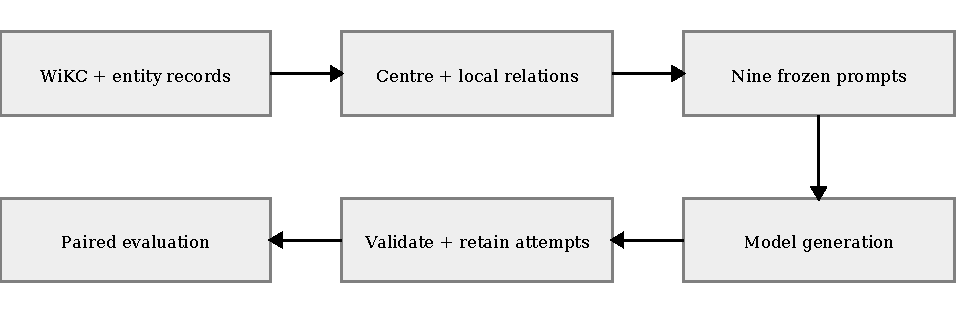
\includegraphics[width=\linewidth]{figures/pipeline.pdf}
\caption{The final generation and evaluation pipeline.}\label{figure:5.1}
\end{figure}

\begingroup
\begin{table}[!htbp]
\setlength{\tabcolsep}{3pt}
\renewcommand{\arraystretch}{1.18}
\fontsize{8.5}{10.5}\selectfont
\renewcommand{\thetable}{5.1}
\renewcommand{\tablename}{Algorithm}
\caption[]{Deterministic oracle context extraction (Definitions 2.5–2.6).}\label{algorithm:5.1}
\begin{tabular}{>{\raggedright\arraybackslash}p{\dimexpr 0.082789\linewidth-2\tabcolsep\relax}>{\raggedright\arraybackslash}p{\dimexpr 0.917211\linewidth-2\tabcolsep\relax}}
\toprule
\textbf{Step} & \textbf{Operation} \\
\midrule
1 & Read all gold identifiers and their annotated depths for entity e. \\
2 & Keep gold classes with no annotated descendant; use all gold classes if this set is empty. \\
3 & Sort by decreasing annotated depth, then ascending identifier string; select c*(e). \\
4 & Find parents, children, and siblings sharing a parent, excluding the centre. Missing graph nodes yield empty lists. \\
5 & Sort each relation list lexicographically and retain its first three identifiers. \\
6 & Render labels for the selected relations; omit the centre label from the context. Keep all gold annotations for evaluation. \\
\bottomrule
\end{tabular}
\end{table}
\endgroup


The omitted centre does not make the context blind to the answer. Its parents and children can strongly constrain the missing class, and the centre is selected using gold annotations. The experiment uses that information to test relevant structure; autonomous deployment would require candidate retrieval without gold access.


\FloatBarrier

\section{Prompt templates and demonstration}

Prompting specifies a task through the text supplied to a language model at inference time. It can describe the required output, provide evidence, and illustrate acceptable behaviour. In-context examples show an input and a desired response without updating model weights. \citet{brown2020} demonstrated the usefulness of this general few-shot setup across language tasks. Here, prompting supplies both the typing instructions and a fixed worked example; no model is fine-tuned on the evaluation entities.


Every final prompt contains one positive demonstration and is therefore one-shot. The external entity is Rod Fergusson (wd:Q18720219), described as a Canadian video game producer, and is outside the 1,000-entity evaluation cohort. The same demonstration entity is used throughout, with condition-specific context and response format. The contrastive style adds an incorrect ranking for that same example; it does not add a second demonstration entity.


Output instructions matter because the model has considerable freedom. The final common instruction requests concise labels, asks for the most specific label first, forbids duplicates and padding, and restricts predictions to evidence-supported types. Graph prompts add a warning that the neighbourhood surrounds an omitted class and is evidence rather than answer options. These instructions address observed tendencies to copy nearby classes, add generic filler, or treat siblings as automatically incompatible.


Prompting remains an empirical design choice. A more elaborate instruction can make the desired behaviour clearer, but it can also alter output length and introduce additional constraints. The study therefore compares fixed templates and retains the generated prompt files. It does not infer that the final wording is optimal. Because the wording was developed using earlier project experience, the full-cohort evaluation is an exploratory assessment of that selected design. A future confirmatory experiment should freeze the templates before opening a new evaluation set.


Chain-of-thought prompting elicits intermediate reasoning before an answer. \citet{wei2022} developed a few-shot formulation in which demonstrations contain reasoning steps as well as final outputs, and evaluated it on reasoning tasks. This motivates an entity-typing prompt that explains why a specific category is supported and how broader categories follow. It does not establish in advance that explanations will improve typing in every model.


The no-graph CoT prompt asks for a brief explanation of the most specific supported type, rejection of unsupported nearby alternatives, and justification of the broader labels and their order. It explicitly limits the evidence to the entity and description. The graph CoT prompt asks the explanation to use parents for semantic scope, compare sibling alternatives, and examine whether child types require unsupported specificity. The output contains an explanation followed by the ordered types list.


This is an adaptation of chain-of-thought prompting to ranked entity typing. “CoT” denotes the explanation-bearing template and demonstration. An explanation is observable output, not a verified account of internal computation: \citet{turpin2023} show that plausible CoT explanations can omit influences on a prediction. Gemini also uses internal thinking under the standard template, so visible explanation and internal reasoning must be distinguished.


Contrastive chain-of-thought prompting adds examples of invalid reasoning alongside valid reasoning. \citet{chia2023} proposed this approach to teach models which mistakes to avoid. The project adapts that principle to entity typing by using a negative demonstration and asking the model to distinguish a supported type from plausible, overly narrow, or incompatible alternatives. The graph version grounds those alternatives in sibling and child relations.


A useful contrast identifies the additional evidence an alternative would require. A class below the centre class may need an attribute absent from the description. A nearby sibling may share a broad parent but describe a different occupation, object, or role. These alternatives can clarify the boundary of a type. However, sibling membership alone does not prove an alternative false. A person can hold several related occupations, and multiple inheritance allows classes to overlap. The final prompt therefore tells the model to reject an alternative only when the evidence warrants rejection.


The contrastive condition is not a reproduction of the original paper’s benchmark or demonstration-construction procedure. It is a task-specific application of learning from correct and incorrect examples. Nor does the presence of sibling labels make every graph prompt formally contrastive: the standard graph prompt also sees siblings, but does not request the same explanation pattern or negative demonstration. These distinctions preserve the meaning of the experimental conditions.


\FloatBarrier

\section{Final prompt conditions and evidence controls}

Table~\ref{table:5.1} defines the nine conditions in Definition 2.9. Standard prompts request a JSON object containing types. CoT and contrastive prompts also request an explanation. Every list is ordered from specific to broad. Appendix C prints all nine complete prompts for framboid, including their actual demonstration text.


\begingroup
\begin{table}[!htbp]
\setlength{\tabcolsep}{3pt}
\renewcommand{\arraystretch}{1.18}
\fontsize{8.5}{10.5}\selectfont
\renewcommand{\thetable}{5.1}
\caption{Nine main conditions and mean Gemini thinking tokens (1,000 completed responses per condition).}\label{table:5.1}
\begin{tabular}{>{\raggedright\arraybackslash}p{\dimexpr 0.261438\linewidth-2\tabcolsep\relax}>{\raggedright\arraybackslash}p{\dimexpr 0.244009\linewidth-2\tabcolsep\relax}>{\raggedright\arraybackslash}p{\dimexpr 0.309368\linewidth-2\tabcolsep\relax}>{\raggedright\arraybackslash}p{\dimexpr 0.185185\linewidth-2\tabcolsep\relax}}
\toprule
\textbf{Condition} & \textbf{Response style} & \textbf{Graph evidence} & \textbf{Gemini thinking tokens} \\
\midrule
Standard no graph & Standard & None & 476.81 \\
Standard graph & Standard & Parents, siblings, children & 849.96 \\
CoT no graph & Explanation & None & 591.17 \\
CoT graph & Explanation & Parents, siblings, children & 1575.32 \\
Contrastive no graph & Contrastive explanation & None & 595.28 \\
Contrastive graph & Contrastive explanation & Parents, siblings, children & 1766.92 \\
Parents only & Standard & Parents & 584.18 \\
Siblings only & Standard & Siblings & 726.71 \\
Children only & Standard & Children & 706.78 \\
\bottomrule
\end{tabular}
\end{table}
\endgroup


Each relation list is capped at three neighbours, selected by ascending identifier string (Definition 2.6). This controls prompt size without semantically ranking neighbours. Empty lists remain visible as absent evidence. Relation-only conditions differ in availability and list length, so they measure implemented prompt configurations rather than an intrinsic causal value of an edge type.


The graph/no-graph contrast changes both evidence and instructions. For example, the standard graph template adds the following note, absent from standard no graph:


\begin{Verbatim}[fontsize=\footnotesize,breaklines=true,breakanywhere=true]
The context surrounds an omitted target type; it is evidence, not answer options. Parents are broader, children narrower, and siblings share a parent. Infer the type using the description and these relations. Copy a neighbour only if valid for this entity. Siblings need not be disjoint; predict a child only when the description independently supports it.
\end{Verbatim}

It also adds taxonomy blocks to the demonstration and test entity. CoT and contrastive conditions change their explanation instructions and worked responses; Appendix C makes those differences explicit. The 549 entities without children support a partial control: children-only versus standard no graph has no test-entity child labels. However, the worked example and graph-related text still differ, so this estimates the whole empty-evidence prompt change, not the graph note in isolation.


The child intervention removes the test child section and the associated child-specific wording from each graph template, while retaining the entity, parents, siblings, and prompting style. It therefore estimates the implemented child-removal treatment, not an evidence-only deletion. Source hashes link each child-removal record to the corresponding main input.


\FloatBarrier

\section{Model systems and generation configuration}

Gemini 3.8 Flash (model ID gemini-3.8-flash) is accessed through the Gemini API generateContent endpoint. \citet{googledeepmind2026} provides its model card. The archived model metadata and API documentation report a 1,048,576-token input limit and a 65,536-token output limit \citep{google2026}. Requests use temperature 1.0, JSON MIME output, and the provider’s default thinking configuration; no thinking override, seed, or maxOutputTokens value is sent.


{\small Archived response timestamps are 11–12 October 2026 for Gemini and 12 October 2026 for all three Llama seeds (UTC).\par}


Gemini supports internal thinking at low, medium, and high levels; standard prompting here means no requested visible explanation, not disabled internal thinking. Table~\ref{table:5.1} reports mean archived thoughtsTokenCount values by condition. These tokens are not an independent measure of reasoning quality.


Llama uses meta-llama/Llama-3.1-8B-Instruct at revision \nolinkurl{0e9e39f249a16976918f6564b8830bc894c89659} \citep{grattafiori2024}. The new run environments record an NVIDIA H100 80GB HBM3 GPU, bfloat16, vLLM 0.31.0, PyTorch 2.13.0, Transformers 5.17.0, and CUDA 13.0. The vLLM release record dates version 0.31.0 to 5 October 2026 \citep{vllmproject2026}, before these runs.


Main Llama runs use seeds 0, 42, and 123; child removal uses seed 0. Temperature 1.0 leaves sampling logits unscaled and provides a common stochastic reference setting across conditions. It was fixed rather than tuned for typing accuracy; the archives do not establish that it is optimal. Three seeds check how sensitive the Llama comparisons are to sampled outputs at this setting, rather than substituting a single greedy response for that protocol. Sampling uses the runner’s top-p default of 1.0. The local context limit is 32,768 tokens; max\_\allowbreak{}new\_\allowbreak{}tokens = 0 in the wrapper allocates the remaining context after the prompt. Batches contain 128 jobs with up to 32 active sequences.


Matching temperature does not make the systems equivalent. Their tokenizers, sampling, model scale, serving systems, and internal thinking differ. RQ4 compares these deployments, while within-model contrasts hold their system-specific configuration fixed.


\FloatBarrier

\section{Failure recovery and response validation}

A completed response must terminate naturally, parse successfully, and contain a nonempty list of type strings; explanation-bearing conditions must also provide a nonempty explanation. JSON-object mode aids syntax without bounding explanation length or list size. Stored predictions are checked against the response and input fingerprints. Completion is a format criterion, not a correctness judgment.


Llama allows at most two generation attempts per job and retries outputs failing validation, including truncation and parsing failures, at the run’s recorded seed. Failed final records are retained. Gemini retries a malformed or truncated output once per invocation when the finish reason is STOP or MAX\_\allowbreak{}TOKENS. Transient network errors and HTTP 429/500/502/503/504 are retried until the fourth transient error; an unresolved response stops new work and can be resumed in a later invocation. The first valid output is retained, with no score-based selection.


The Gemini external-demonstration run contains 9,000 completed final outputs and archived attempts. Table~\ref{table:5.2} summarizes first recorded attempt validity and final validity; accepted attempts also saved as final records are deduplicated. Table~\ref{table:A.7} gives condition-level retry counts.


\begingroup
\begin{table}[!htbp]
\setlength{\tabcolsep}{3pt}
\renewcommand{\arraystretch}{1.18}
\fontsize{8.5}{10.5}\selectfont
\renewcommand{\thetable}{5.2}
\caption{Run-level validity and retry summary.}\label{table:5.2}
\begin{tabular}{>{\raggedright\arraybackslash}p{\dimexpr 0.355120\linewidth-2\tabcolsep\relax}>{\raggedright\arraybackslash}p{\dimexpr 0.161220\linewidth-2\tabcolsep\relax}>{\raggedright\arraybackslash}p{\dimexpr 0.161220\linewidth-2\tabcolsep\relax}>{\raggedright\arraybackslash}p{\dimexpr 0.161220\linewidth-2\tabcolsep\relax}>{\raggedright\arraybackslash}p{\dimexpr 0.161220\linewidth-2\tabcolsep\relax}}
\toprule
\textbf{Run} & \textbf{Jobs} & \textbf{First valid} & \textbf{Retried jobs} & \textbf{Final valid} \\
\midrule
Gemini & 9000 & 8982 & 18 & 9000 \\
Llama 0 & 9000 & 8969 & 31 & 8991 \\
Llama 42 & 9000 & 8929 & 71 & 8971 \\
Llama 123 & 9000 & 8963 & 37 & 8986 \\
Llama 0 child removal & 1353 & 1347 & 6 & 1352 \\
\bottomrule
\end{tabular}
\end{table}
\endgroup


Main Llama runs have 9, 29, and 14 failed outputs at seeds 0, 42, and 123; child removal completes 1,352/1,353 responses. Primary contrasts use paired completed responses, and seed comparisons use common completed cohorts. Section 7.2 reports the zero-for-failure sensitivity check.


Retry rates vary by condition. Table~\ref{table:A.7} provides the detailed counts and duplicate-key parsing convention, which qualify accepted-response comparisons.


\FloatBarrier

\section{Development history}

Early prompt versions explored standard responses, explanation-bearing responses, contrastive examples, and alternative context selection. Inspection of exploratory outputs informed the compact wording and specific-to-broad output instructions. Those earlier model results are excluded from every score in this thesis. Previously exposed evaluation entities remain in the cohort, so the final analysis is exploratory.


The author also explored deriving taxonomy structure from the dataset using an LLM. The additional generated structure did not offer a sufficiently clear practical improvement to retain it. This was a development assessment, not a measured information-theoretic result or a controlled extraction benchmark. A fixed WiKC resource was chosen so that relation selection and downstream typing could be inspected separately.


\chapter{Evaluation design}

\FloatBarrier

\section{Precision, recall, and entity F1}

Set metrics follow Definition 2.10 and the normalization in Definition 2.8. For each entity, \ensuremath{\hat{P}} contains unique normalized predicted labels and \ensuremath{\hat{G}} contains unique normalized gold labels. True positives are their intersection. Precision measures predicted-label agreement, recall measures gold recovery, and F1 balances both. The same full gold set is used in every condition.


Precision = |\ensuremath{\hat{P}} \ensuremath{\cap} \ensuremath{\hat{G}}| / |\ensuremath{\hat{P}}|; recall = |\ensuremath{\hat{P}} \ensuremath{\cap} \ensuremath{\hat{G}}| / |\ensuremath{\hat{G}}|;\par F1(e) = 2|\ensuremath{\hat{P}} \ensuremath{\cap} \ensuremath{\hat{G}}| / (|\ensuremath{\hat{P}}| + |\ensuremath{\hat{G}}|); macro F1 = mean\textsubscript{e} F1(e).


Normalization applies the historical scorer’s lowercasing, whitespace and underscore handling, and surrounding-punctuation cleanup. It does not introduce semantic aliases. Duplicate predictions count once in the set metrics. Empty predictions would receive zero, although accepted-response scoring requires a nonempty types list. The macro-F1 reported in the thesis is the arithmetic mean of entity F1 scores, giving each entity equal weight.


Multi-label entity typing literature uses several aggregation conventions \citep{choi2018}. To avoid ambiguity, the project also exports micro scores obtained from pooled counts and a separate loose macro-F1 formed by taking the harmonic mean of mean precision and mean recall. These values are not interchangeable with the mean of entity F1. The figures and principal comparisons consistently use the latter.


This choice prevents entities with very long annotation chains from automatically dominating the headline score. It also makes the paired contrast intuitive: each entity contributes its own graph-induced score change. However, exact-label matching penalizes synonyms and descriptions that are not in the source inventory. A label can be plausible in ordinary language yet be counted as a false positive. The thesis therefore describes the metric as benchmark agreement rather than an exhaustive semantic correctness judgment.


Precision and recall are shown separately because an F1 increase can arise in different ways. A model may become more selective, recover additional ancestors, or do both. Output length is retained as a diagnostic rather than rewarded by itself. A graph prompt that merely adds many types would be expected to improve some coverage while risking lower precision. The actual results improve both metrics in all primary contrasts, which makes a simple list-expansion explanation insufficient.


Strict accuracy is also available in the archive. It requires the predicted set to equal the entire gold set. This is demanding for long hierarchies and open-vocabulary output, so it is a supporting diagnostic rather than the only success criterion. The main evaluation preserves a distinction between partial but useful recovery and complete reconstruction.


\FloatBarrier

\section{Ranking and maximum-depth gold-label recovery}

Ranking follows Definition 2.11. MRR evaluates the first occurrence of any label in Gmax(e), not necessarily the context centre c*(e) from Definition 2.5. The distinction matters because shortest-path depth and graph-minimality can disagree. A first matching rank j receives reciprocal rank 1/j; a miss receives zero.


Normalized discounted cumulative gain provides graded credit for the whole ordered list. Following the gain-and-discount framework of \citet{jarvelin2002}, the project assigns each gold label a relevance equal to its annotated depth divided by the maximum gold depth. Unmatched labels receive zero. The exponential gain is 2 raised to that relevance minus one, and the rank discount is the base-2 logarithm of rank plus one. The ideal list sorts all gold relevance values in descending order.


The full-list implementation sets its evaluation length to the larger of prediction length, gold-label count, and one. Missing positions are padded with zero relevance. A repeated matched label earns relevance only on its first credited occurrence, preventing repeated labels from inflating gain. The root at depth zero receives zero relevance when a deeper class exists. These choices are project-specific adaptations of a general ranking metric, not a canonical entity-typing standard imposed by the cited paper.


MRR asks whether the maximum-depth gold label is early. nDCG asks whether the list places deeper gold labels ahead of weaker or unmatched labels. Recall asks how many gold labels occur anywhere. A condition can therefore improve nDCG substantially while changing MRR only slightly, as observed in Llama. That pattern is consistent with better ordering or recovery of intermediate gold classes without equally large improvement in the maximum-depth gold label.


The analysis also reports maximum-depth hit rate, which ignores the rank of a recovered maximum-depth gold label, and bins recovery into first rank, second rank, later rank, or miss. These diagnostics explain where MRR differences arise. They do not introduce alternative gold answers. The same normalization and annotated hierarchy are used throughout, so the ranking results remain tied to the benchmark vocabulary and its depth convention.


\FloatBarrier

\section{Hierarchy diagnostics and interpretable errors}

Flat matching treats every wrong label alike, even though a nearby ancestor and an unrelated class have different structural relationships to gold. Hierarchical evaluation research emphasizes that these relationships and the choice of augmentation affect the score (Kosmopoulos et al., 2015; Plaud et al., 2024). The project therefore adds ancestor-augmented hierarchical F1, error direction, graph distance, and hierarchy consistency.


For hierarchical F1, each mapped class is expanded to include itself and all reachable ancestors, including roots. Precision, recall, and F1 are then computed over these expanded sets. All parents in the acyclic graph are considered. A label matching an annotated gold label resolves to its annotated class identifiers. Otherwise, only a unique normalized class-label mapping resolves. Unmapped or ambiguous predictions remain opaque false-positive items; they are not silently removed from the denominator.


This metric gives credit for related structure but has limitations. Common ancestors can make scores high even when specific labels are wrong. It also uses gold information to disambiguate exact gold-label matches. Its values must be interpreted alongside flat F1 and maximum-depth gold-label recovery. The implementation is ancestor-closure hierarchical F1, not the separate lowest-common-ancestor F1 algorithm discussed by \citet{kosmopoulos2015}.


For each mapped incorrect prediction, error distance is the minimum undirected shortest-path distance to any annotated gold class. Unmapped, ambiguous, disconnected, or absent nodes have no finite distance and are reported separately. Because the gold set contains broad ancestors, the nearest gold node can be broad; a short distance does not prove that the prediction is near the most specific answer. Pooling errors and averaging within-entity distances also produce different estimands, so their denominators are retained in the output tables.


Directional categories use an explicit precedence: exact gold, broader, narrower, sibling, then other taxonomy relationships. This resolves overlaps in a graph where a prediction may relate differently to several gold branches. Hierarchy consistency asks whether every ancestor of a resolved predicted node already appears in the unaugmented output. It is undefined for entities without resolved graph nodes, and eligible counts are reported.


Consistency is not correctness. A model can be internally closed over the wrong branch, while a concise correct answer can omit broad ancestors and score poorly on consistency. The diagnostics are therefore used to characterize behaviour and identify cases for inspection. They complement the five primary requested metrics rather than replace them with a single structural score.


\FloatBarrier

\section{Worked metric example}

Consider a small illustrative taxonomy with cat \ensuremath{\to} mammal \ensuremath{\to} animal \ensuremath{\to} entity and dog \ensuremath{\to} mammal. Let the listed gold labels be \{cat, mammal, animal, entity\}, with depths 3, 2, 1, 0. Suppose the ranked prediction is [mammal, dog, cat]. This example illustrates the metrics rather than reporting an experimental result.


\begingroup
\begin{table}[!htbp]
\setlength{\tabcolsep}{3pt}
\renewcommand{\arraystretch}{1.18}
\fontsize{8.5}{10.5}\selectfont
\renewcommand{\thetable}{6.1}
\caption{Scores for the worked example.}\label{table:6.1}
\begin{tabular}{>{\raggedright\arraybackslash}p{\dimexpr 0.224401\linewidth-2\tabcolsep\relax}>{\raggedright\arraybackslash}p{\dimexpr 0.623094\linewidth-2\tabcolsep\relax}>{\raggedright\arraybackslash}p{\dimexpr 0.152505\linewidth-2\tabcolsep\relax}}
\toprule
\textbf{Metric} & \textbf{Calculation} & \textbf{Value} \\
\midrule
Precision & 2 matching labels / 3 predictions & 0.6667 \\
Recall & 2 matching labels / 4 gold labels & 0.5000 \\
Entity F1 & 2 \ensuremath{\times} 2 / (3 + 4) & 0.5714 \\
Reciprocal rank & cat first occurs at rank 3 & 0.3333 \\
DCG & (2\textasciicircum{}(2/3) \ensuremath{-} 1) + 1/log\textsubscript{2}(4) & 1.0874 \\
IDCG & 1 + (2\textasciicircum{}(2/3) \ensuremath{-} 1)/log\textsubscript{2}(3) + (2\textasciicircum{}(1/3) \ensuremath{-} 1)/log\textsubscript{2}(4) & 1.5006 \\
nDCG & DCG / IDCG & 0.7247 \\
Hierarchical F1 & Expanded prediction has 5 nodes; gold has 4; overlap is 4 & 0.8889 \\
\bottomrule
\end{tabular}
\end{table}
\endgroup


Table~\ref{table:6.1} illustrates the metric calculations. The ranking penalty reflects the delayed cat label; the set metrics also penalize dog and missing ancestors. Ancestor augmentation recovers mammal, animal, and entity, so hierarchical F1 is higher. That higher score does not make dog a correct flat prediction.


\FloatBarrier

\section{Paired uncertainty and visual presentation}

The primary comparison aligns two outputs for the same entity, within the same model and prompting style. Each entity contributes a difference, such as graph F1 minus no-graph F1. The reported effect is the mean of those paired differences. This avoids a comparison of unrelated groups and retains the dependence induced by shared descriptions and annotations. Statistical testing guidance in NLP stresses matching the procedure to the experimental unit and metric \citep{dror2018}.


Confidence intervals use 2,000 paired bootstrap resamples of entities with seed 230917. The 2.5th and 97.5th percentiles form the displayed 95\% interval. The same approach supports the child intervention and model score differences and differences between model-specific graph gains. Resampling entity differences retains the pairing. It does not resample individual generated labels as if they were independent observations.


Each primary contrast uses entities with completed responses in both conditions. Child comparisons similarly intersect the eligible cohort with both completed outputs. For between-seed condition comparisons, all three Llama seeds use the same completed entities. Gemini-versus-seed comparisons align entities within each condition. Pairwise denominators are printed; this prevents unmatched cohort means from being interpreted as paired effects.


Between-seed means and sample standard deviations use the three condition means on the common cohort, with standard-deviation divisor 3 \ensuremath{-} 1. They describe observed variation across three seeds, not a precise population estimate. A completion-inclusive sensitivity analysis assigns failed responses zero and uses all 1,000 planned entities; this is explicitly separated from accepted-response scoring.


The intervals are exploratory and uncorrected for multiple comparisons. They describe variation over entities in this cohort under the accepted outputs. They do not cover API drift, choice of demonstrations, repeated inference seeds, prompt selection, or all uncertainty in benchmark annotations. An interval excluding zero is consequently evidence of a consistent cohort effect under this protocol, not a universal performance guarantee. Helped, tied, and harmed counts accompany the means; ties use an absolute difference threshold of 10\textsuperscript{-12}.


Figures and tables centre on matched graph-versus-no-graph contrasts within each prompting style. Every plotted bar has a numerical value rounded to four decimals. Tables give the corresponding paired effects, intervals, sample sizes, and output lengths. Condition means, paired differences, and seed variation are identified separately.


\citet{cleveland1984} motivate accurate comparisons through position and length on common scales. \citet{ho2019} motivate showing effect magnitudes and uncertainty instead of reducing interpretation to a significance label. The thesis applies these principles with restrained colours, explicit legends, readable labels, and numerical tables. Dense distributions are shown as labelled cells rather than stacks whose internal segments are difficult to compare.


Entity distribution tables provide context for interpretation, while the main performance plots remain centred on structural evidence. This organization follows the research question: whether graph context helps, how the effect differs by prompting style, and what the ablations reveal. The model comparison follows these primary findings so that it does not displace the thesis’s focal contribution.


\chapter{Results}

\FloatBarrier

\section{Graph-aware prompting improves F1, precision, and recall}

RQ1 is answered by the three within-model contrasts. Figure~\ref{figure:7.1} shows paired-cohort F1 values, and Table~\ref{table:A.4} reports per-seed graph minus no-graph effects and intervals. All twelve F1 effects are positive, including each of the three Llama seeds. The treatment includes graph evidence and its interpretation instructions.


\begin{figure}[htbp]
\centering
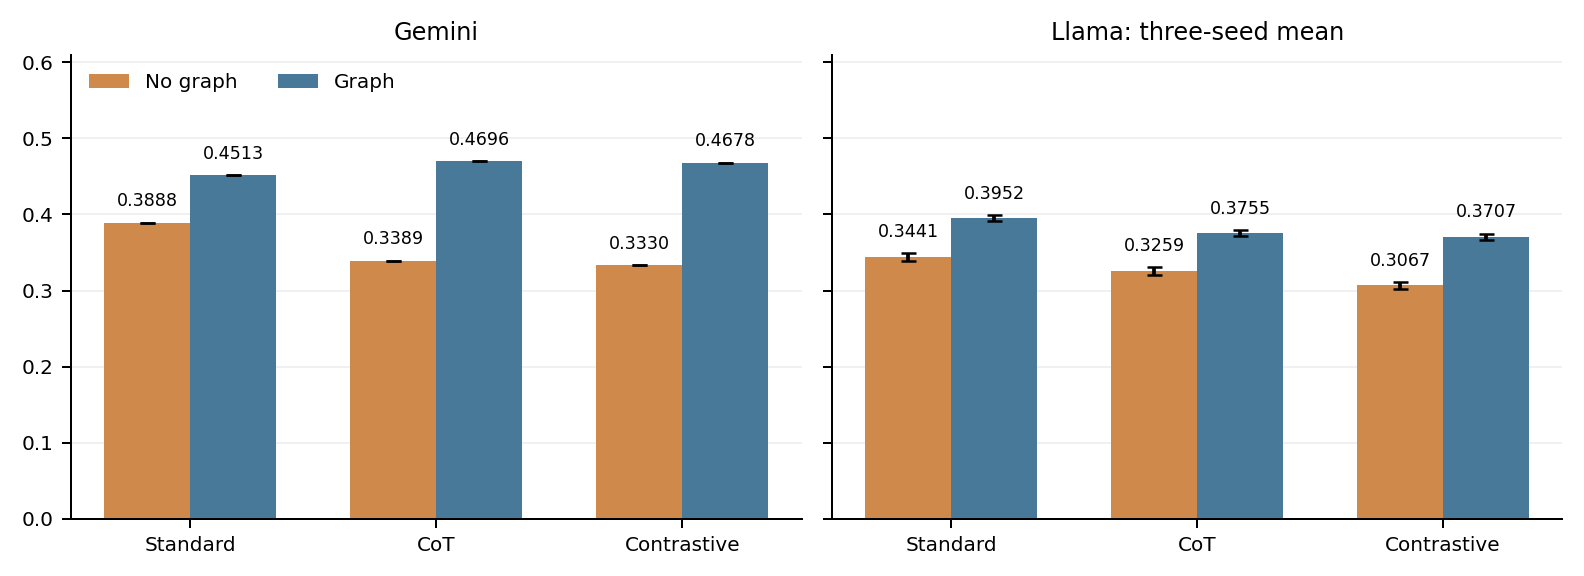
\includegraphics[width=\linewidth]{figures/f1.png}
\caption{Mean entity F1 on each matched graph/no-graph cohort; Gemini and the Llama seed mean; error bars show sample SD across three seed means. Paired effects and n are in Table~\ref{table:A.4}.}\label{figure:7.1}
\end{figure}

Parents expose broader category vocabulary and neighbours constrain the intended branch, which can improve both selecting and ordering labels. These are plausible explanations, not isolated causal mechanisms: the added graph note and worked-example wording also contribute to the treatment.


\subsection*{Precision, recall, and description overlap}

Table~\ref{table:7.1} reports precision, recall, and generated-label counts. Llama means use the same entities across all three seeds and both conditions within each style.


\begingroup
\begin{table}[!htbp]
\setlength{\tabcolsep}{3pt}
\renewcommand{\arraystretch}{1.18}
\fontsize{8.5}{10.5}\selectfont
\renewcommand{\thetable}{7.1}
\caption{Precision, recall, and generated labels; N/G denote no graph/graph.}\label{table:7.1}
\begin{tabular}{>{\raggedright\arraybackslash}p{\dimexpr 0.254902\linewidth-2\tabcolsep\relax}>{\raggedright\arraybackslash}p{\dimexpr 0.117647\linewidth-2\tabcolsep\relax}>{\raggedright\arraybackslash}p{\dimexpr 0.117647\linewidth-2\tabcolsep\relax}>{\raggedright\arraybackslash}p{\dimexpr 0.117647\linewidth-2\tabcolsep\relax}>{\raggedright\arraybackslash}p{\dimexpr 0.117647\linewidth-2\tabcolsep\relax}>{\raggedright\arraybackslash}p{\dimexpr 0.137255\linewidth-2\tabcolsep\relax}>{\raggedright\arraybackslash}p{\dimexpr 0.137255\linewidth-2\tabcolsep\relax}}
\toprule
\textbf{Model/style} & \textbf{P N} & \textbf{P G} & \textbf{R N} & \textbf{R G} & \textbf{Labels N} & \textbf{Labels G} \\
\midrule
Gemini Standard & 0.4714 & 0.5628 & 0.3503 & 0.3968 & 8.3930 & 8.0630 \\
Gemini CoT & 0.4740 & 0.6116 & 0.2782 & 0.4000 & 6.6190 & 7.4150 \\
Gemini Contrastive & 0.4708 & 0.6120 & 0.2704 & 0.3969 & 6.4840 & 7.3540 \\
Llama mean Standard & 0.3961 & 0.4651 & 0.3391 & 0.3767 & 10.8184 & 9.7018 \\
Llama mean CoT & 0.3710 & 0.4296 & 0.3191 & 0.3677 & 9.9455 & 10.0369 \\
Llama mean Contrastive & 0.3536 & 0.4367 & 0.2959 & 0.3539 & 9.7305 & 9.5712 \\
\bottomrule
\end{tabular}
\end{table}
\endgroup


Precision and recall improve together in all twelve primary contrasts, so list expansion alone does not explain the gains. Figure~\ref{figure:7.2} shows that standard graph outputs are shorter. Gemini CoT lists grow from 6.619 to 7.415 labels (+0.796), and contrastive lists from 6.484 to 7.354 (+0.870), whereas standard lists shrink by 0.330. Explanation-bearing gains therefore combine greater coverage with improved precision. Counts retain repetitions; set scoring deduplicates normalized labels.


\begin{figure}[htbp]
\centering
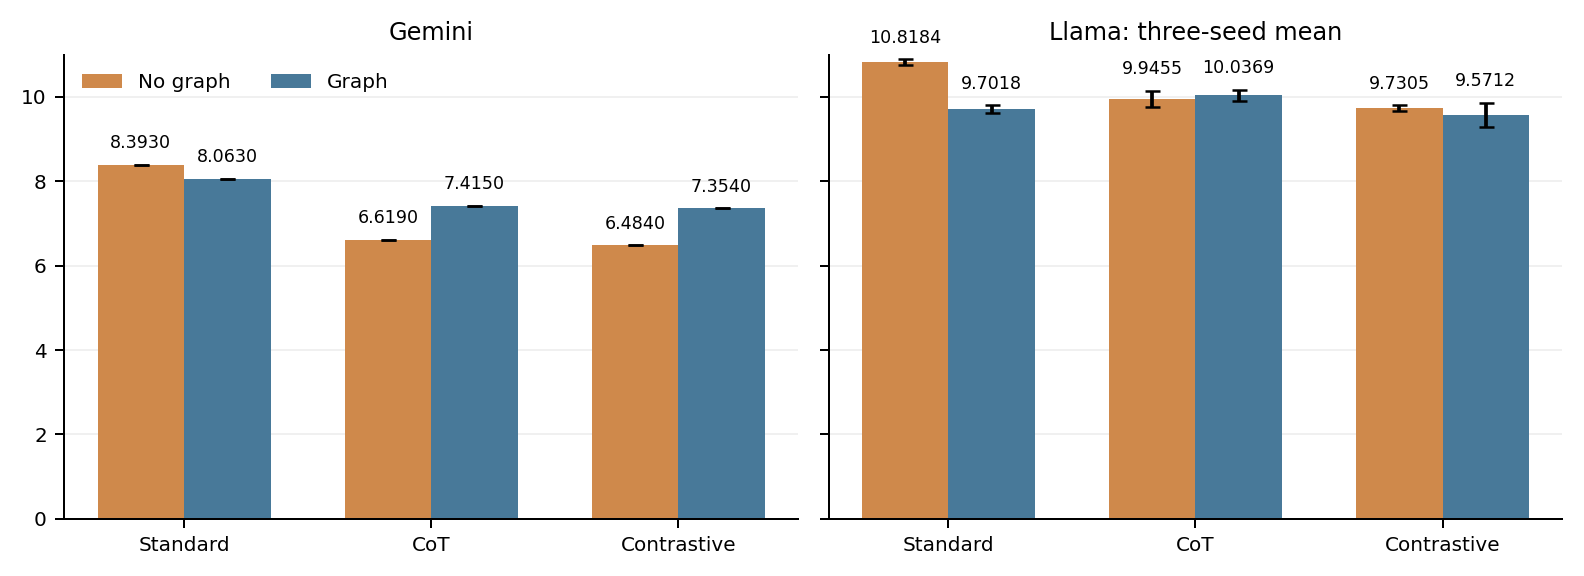
\includegraphics[width=\linewidth]{figures/length.png}
\caption{Mean generated type-label count on matched cohorts; Llama error bars are the SD of three seed means.}\label{figure:7.2}
\end{figure}

Table~\ref{table:7.2} separates effects according to literal centre-label occurrence in the description.


\begingroup
\begin{table}[!htbp]
\setlength{\tabcolsep}{3pt}
\renewcommand{\arraystretch}{1.18}
\fontsize{8.5}{10.5}\selectfont
\renewcommand{\thetable}{7.2}
\caption{Paired F1 gains by literal centre-label occurrence in the description.}\label{table:7.2}
\begin{tabular}{>{\raggedright\arraybackslash}p{\dimexpr 0.355120\linewidth-2\tabcolsep\relax}>{\raggedright\arraybackslash}p{\dimexpr 0.161220\linewidth-2\tabcolsep\relax}>{\raggedright\arraybackslash}p{\dimexpr 0.161220\linewidth-2\tabcolsep\relax}>{\raggedright\arraybackslash}p{\dimexpr 0.161220\linewidth-2\tabcolsep\relax}>{\raggedright\arraybackslash}p{\dimexpr 0.161220\linewidth-2\tabcolsep\relax}}
\toprule
\textbf{Model/style} & \textbf{Present n} & \textbf{Gain} & \textbf{Absent n} & \textbf{Gain} \\
\midrule
Gemini Standard & 265 & +0.0591 & 735 & +0.0637 \\
Gemini CoT & 265 & +0.0967 & 735 & +0.1431 \\
Gemini Contrastive & 265 & +0.1095 & 735 & +0.1439 \\
Llama 0 Standard & 265 & +0.0537 & 735 & +0.0615 \\
Llama 0 CoT & 265 & +0.0395 & 734 & +0.0599 \\
Llama 0 Contrastive & 263 & +0.0524 & 732 & +0.0642 \\
Llama 42 Standard & 265 & +0.0558 & 733 & +0.0454 \\
Llama 42 CoT & 260 & +0.0394 & 731 & +0.0499 \\
Llama 42 Contrastive & 264 & +0.0650 & 727 & +0.0606 \\
Llama 123 Standard & 263 & +0.0365 & 734 & +0.0482 \\
Llama 123 CoT & 263 & +0.0589 & 732 & +0.0435 \\
Llama 123 Contrastive & 263 & +0.0582 & 732 & +0.0737 \\
\bottomrule
\end{tabular}
\end{table}
\endgroup


The gains in the label-absent group directly address the running-example concern: graph-aware prompting is useful beyond descriptions that literally name the selected centre. This split is descriptive, because lexical overlap also co-varies with entity categories, gold-list length, and available context.


Table~\ref{table:A.4} reports helped, tied, and harmed counts for all twelve style/run contrasts. A positive mean does not imply a benefit for every entity.


\FloatBarrier

\section{Variation across the three Llama seeds}

The three seeds assess the stability of the Llama results supporting RQ1 and RQ4. Table~\ref{table:7.3} uses one common completed cohort per condition, so seed variation is not caused by different entity membership. The standard graph condition has the largest F1 among the three combined-graph styles at every seed, while the relation-only results vary more.


\begingroup
\begin{table}[!htbp]
\setlength{\tabcolsep}{3pt}
\renewcommand{\arraystretch}{1.18}
\fontsize{8.5}{10.5}\selectfont
\renewcommand{\thetable}{7.3}
\caption{Llama F1 variability on common completed entities; sample SD across three seed means.}\label{table:7.3}
\begin{tabular}{>{\raggedright\arraybackslash}p{\dimexpr 0.607843\linewidth-2\tabcolsep\relax}>{\raggedright\arraybackslash}p{\dimexpr 0.196078\linewidth-2\tabcolsep\relax}>{\raggedright\arraybackslash}p{\dimexpr 0.196078\linewidth-2\tabcolsep\relax}}
\toprule
\textbf{Condition} & \textbf{n} & \textbf{SD} \\
\midrule
Standard no graph & 1000 & 0.0047 \\
Standard graph & 995 & 0.0039 \\
CoT no graph & 994 & 0.0053 \\
CoT graph & 991 & 0.0039 \\
Contrastive no graph & 991 & 0.0046 \\
Contrastive graph & 990 & 0.0041 \\
Parents only & 997 & 0.0218 \\
Siblings only & 993 & 0.0119 \\
Children only & 997 & 0.0160 \\
\bottomrule
\end{tabular}
\end{table}
\endgroup


Parent-only F1 is more variable than the combined standard graph result. It exceeds the combined-context F1 at seeds 0 and 42 but falls below it at seed 123. Combined context supplies several kinds of evidence, which may reduce dependence on an individual relation list; parent-only responses can instead be more sensitive to sampled choices of broad labels. This is a possible explanation for the observed variability, not a tested mechanism. The stable combined-style ordering supports that comparison more strongly than selecting one best relation condition from a single seed.


With failures assigned zero across all 1,000 entities, all nine Llama graph gains remain positive, from +0.0437 to +0.0702. Incomplete outputs do not change the direction of RQ1, although accepted-response means remain conditional on validation and retries.


\FloatBarrier

\section{Maximum-depth gold-label ranking and graded list quality}

RQ1 also concerns ranked output. Figure~\ref{figure:7.3} shows MRR, and Table~\ref{table:7.4} gives paired gains in MRR and nDCG. Both increase in every model-by-style contrast. Gemini’s ranking gains are larger than Llama’s, especially under the explanation-bearing templates.


\begin{figure}[htbp]
\centering
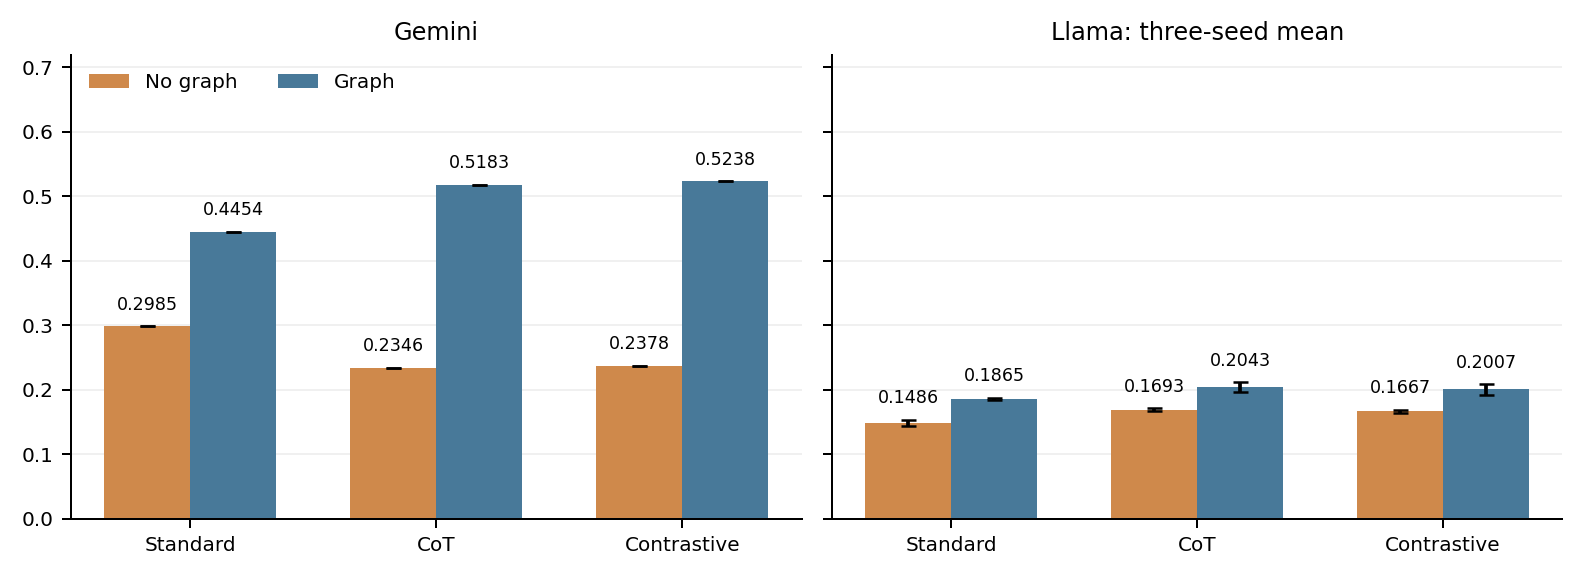
\includegraphics[width=\linewidth]{figures/mrr.png}
\caption{Maximum-depth gold-label MRR, using matched successful responses. Llama is summarized by the three-seed mean with sample SD.}\label{figure:7.3}
\end{figure}

\begingroup
\begin{table}[!htbp]
\setlength{\tabcolsep}{3pt}
\renewcommand{\arraystretch}{1.18}
\fontsize{8.5}{10.5}\selectfont
\renewcommand{\thetable}{7.4}
\caption{Paired graph gains in MRR and depth-weighted nDCG.}\label{table:7.4}
\begin{tabular}{>{\raggedright\arraybackslash}p{\dimexpr 0.542484\linewidth-2\tabcolsep\relax}>{\raggedright\arraybackslash}p{\dimexpr 0.228758\linewidth-2\tabcolsep\relax}>{\raggedright\arraybackslash}p{\dimexpr 0.228758\linewidth-2\tabcolsep\relax}}
\toprule
\textbf{Model/style} & \textbf{MRR gain} & \textbf{nDCG gain} \\
\midrule
Gemini Standard & +0.1469 & +0.1423 \\
Gemini CoT & +0.2837 & +0.2319 \\
Gemini Contrastive & +0.2860 & +0.2342 \\
Llama 0 Standard & +0.0402 & +0.1353 \\
Llama 0 CoT & +0.0281 & +0.1257 \\
Llama 0 Contrastive & +0.0439 & +0.1288 \\
Llama 42 Standard & +0.0445 & +0.1384 \\
Llama 42 CoT & +0.0440 & +0.1315 \\
Llama 42 Contrastive & +0.0309 & +0.1271 \\
Llama 123 Standard & +0.0304 & +0.1302 \\
Llama 123 CoT & +0.0329 & +0.1198 \\
Llama 123 Contrastive & +0.0261 & +0.1289 \\
\bottomrule
\end{tabular}
\end{table}
\endgroup


Table~\ref{table:A.2} reports maximum-depth hit rate, rank bins, strict accuracy, micro-F1, hierarchical F1, and hierarchy consistency. Table~\ref{table:A.3} reports error distance and direction, with explicit denominators. These diagnostics distinguish recovering labels, ranking them early, and generating an ancestor-closed list.


For standard prompting, maximum-depth hit rate rises from 0.4200 to 0.5930 for Gemini and from 0.1850 to 0.2610 for Llama seed 0 (Table~\ref{table:A.2b}). Exact reconstruction remains rare: strict accuracy is 0.0010 in both Gemini conditions and zero in both Llama seed-0 conditions. Hierarchy consistency falls from 0.3282 to 0.2380 for Gemini and from 0.5479 to 0.4298 for Llama seed 0, despite higher hierarchical F1 (Table~\ref{table:A.2a}). Closer ancestor-augmented agreement therefore does not imply a more explicitly closed output list.


Llama’s nDCG gain is consistently larger than its MRR gain. This is consistent with recovering or ordering intermediate gold classes more successfully than recovering a maximum-depth label early. The graph can supply broad vocabulary directly, while identifying the omitted centre still requires interpreting the description and relations. These output patterns do not establish an internal reasoning route.


Selecting a best prompt depends on the metric. The standard graph prompt leads Llama’s combined-context F1 across seeds, while its maximum-depth ranking can favour an explanation-bearing condition. Gemini’s CoT and contrastive graph scores are close; their small differences should not be treated as a general superiority claim.


\FloatBarrier

\section{Relation ablations and model comparison}

RQ2 and H1 concern the relative usefulness of relation conditions. Table~\ref{table:7.5} reports paired gains over standard no graph; full condition scores are in Table~\ref{table:A.1}. Parent-only F1 exceeds sibling-only F1 for Gemini and all Llama seeds, so H1 is not supported. Combined standard context exceeds every single-relation condition for Gemini, but not for Llama seeds 0 and 42.


\begingroup
\begin{table}[!htbp]
\setlength{\tabcolsep}{3pt}
\renewcommand{\arraystretch}{1.18}
\fontsize{8.5}{10.5}\selectfont
\renewcommand{\thetable}{7.5}
\caption{Paired standard-style F1 gains over no graph.}\label{table:7.5}
\begin{tabular}{>{\raggedright\arraybackslash}p{\dimexpr 0.311547\linewidth-2\tabcolsep\relax}>{\raggedright\arraybackslash}p{\dimexpr 0.172113\linewidth-2\tabcolsep\relax}>{\raggedright\arraybackslash}p{\dimexpr 0.172113\linewidth-2\tabcolsep\relax}>{\raggedright\arraybackslash}p{\dimexpr 0.172113\linewidth-2\tabcolsep\relax}>{\raggedright\arraybackslash}p{\dimexpr 0.172113\linewidth-2\tabcolsep\relax}}
\toprule
\textbf{Condition} & \textbf{Gemini} & \textbf{Llama 0} & \textbf{Llama 42} & \textbf{Llama 123} \\
\midrule
Parents only & +0.0414 & +0.0638 & +0.0598 & +0.0213 \\
Siblings only & +0.0070 & +0.0024 & +0.0162 & +0.0014 \\
Children only & +0.0272 & +0.0119 & +0.0204 & -0.0092 \\
Standard graph & +0.0625 & +0.0594 & +0.0482 & +0.0451 \\
\bottomrule
\end{tabular}
\end{table}
\endgroup


Parent labels often belong to the gold ancestor chain, so their utility includes direct access to broader valid vocabulary. Siblings generally do not provide that same immediate overlap. Differences in relation availability and context size also matter. The ablations therefore identify useful prompt configurations rather than proving that parent edges are intrinsically superior in every setting.


Sibling-only context can still assist the more specific ranking task: Gemini’s sibling-only MRR is 0.4316, compared with 0.2985 without graph. A relation may aid identifying a particular class without recovering enough of the broader gold hierarchy to maximize F1.


\begingroup
\begin{table}[!htbp]
\setlength{\tabcolsep}{3pt}
\renewcommand{\arraystretch}{1.18}
\fontsize{8.5}{10.5}\selectfont
\renewcommand{\thetable}{7.6}
\caption{Empty-child partial control: children-only minus standard no graph on entities without test child context.}\label{table:7.6}
\begin{tabular}{>{\raggedright\arraybackslash}p{\dimexpr 0.196078\linewidth-2\tabcolsep\relax}>{\raggedright\arraybackslash}p{\dimexpr 0.076253\linewidth-2\tabcolsep\relax}>{\raggedright\arraybackslash}p{\dimexpr 0.152505\linewidth-2\tabcolsep\relax}>{\raggedright\arraybackslash}p{\dimexpr 0.152505\linewidth-2\tabcolsep\relax}>{\raggedright\arraybackslash}p{\dimexpr 0.141612\linewidth-2\tabcolsep\relax}>{\raggedright\arraybackslash}p{\dimexpr 0.281046\linewidth-2\tabcolsep\relax}}
\toprule
\textbf{Model} & \textbf{n} & \textbf{Standard} & \textbf{Child-only} & \textbf{Gain} & \textbf{95\% interval} \\
\midrule
Gemini & 549 & 0.3840 & 0.4084 & +0.0243 & [+0.0160, +0.0331] \\
Llama 0 & 549 & 0.3352 & 0.3485 & +0.0133 & [+0.0014, +0.0255] \\
Llama 42 & 548 & 0.3452 & 0.3622 & +0.0170 & [+0.0059, +0.0287] \\
Llama 123 & 548 & 0.3367 & 0.3417 & +0.0049 & [-0.0067, +0.0171] \\
\bottomrule
\end{tabular}
\end{table}
\endgroup


Table~\ref{table:7.6} shows small positive point estimates, approximately +0.005 to +0.024, but the Llama seed-123 interval includes zero and seed 0 only narrowly excludes it. This is suggestive evidence of a template contribution, not a uniformly established positive instruction effect. Gemini’s effect is about +0.02 compared with its +0.0625 full-cohort standard graph gain. Because the cohorts and prompt changes differ, this is an indicative comparison, not an estimate of the fraction attributable to the template.


The test child lists are empty for these 549 entities. The comparison measures the empty-evidence prompt package, which still changes graph instructions and the demonstration. It therefore helps assess instruction/template effects but does not isolate the graph note alone. The full graph gains should not be attributed entirely to structural evidence.


RQ4 compares Gemini with each Llama seed on shared completed entities, condition by condition. Table~\ref{table:7.7} summarizes Gemini minus Llama F1 averaged over seeds; Table~\ref{table:A.5} gives every per-seed interval and model difference in graph gains. Positive values favour Gemini; all nine conditions favour Gemini against each seed. This is a comparison of the recorded systems, including Gemini’s default internal thinking, not a controlled test of model architecture.


\begingroup
\begin{table}[!htbp]
\setlength{\tabcolsep}{3pt}
\renewcommand{\arraystretch}{1.18}
\fontsize{8.5}{10.5}\selectfont
\renewcommand{\thetable}{7.7}
\caption{Gemini minus the mean of three Llama seeds, on common completed entities.}\label{table:7.7}
\begin{tabular}{>{\raggedright\arraybackslash}p{\dimexpr 0.389978\linewidth-2\tabcolsep\relax}>{\raggedright\arraybackslash}p{\dimexpr 0.087146\linewidth-2\tabcolsep\relax}>{\raggedright\arraybackslash}p{\dimexpr 0.217865\linewidth-2\tabcolsep\relax}>{\raggedright\arraybackslash}p{\dimexpr 0.305011\linewidth-2\tabcolsep\relax}}
\toprule
\textbf{Condition} & \textbf{n} & \textbf{F1 difference} & \textbf{95\% interval} \\
\midrule
Standard no graph & 1000 & +0.0443 & [+0.0367, +0.0520] \\
Standard graph & 995 & +0.0556 & [+0.0468, +0.0649] \\
CoT no graph & 994 & +0.0131 & [+0.0056, +0.0211] \\
CoT graph & 991 & +0.0949 & [+0.0857, +0.1042] \\
Contrastive no graph & 991 & +0.0264 & [+0.0199, +0.0333] \\
Contrastive graph & 990 & +0.0970 & [+0.0886, +0.1053] \\
Parents only & 997 & +0.0377 & [+0.0294, +0.0458] \\
Siblings only & 993 & +0.0450 & [+0.0359, +0.0539] \\
Children only & 997 & +0.0640 & [+0.0552, +0.0727] \\
\bottomrule
\end{tabular}
\end{table}
\endgroup


Gemini graph prompts use about 1.8, 2.7, and 3.0 times as many thinking tokens as their no-graph counterparts for standard, CoT, and contrastive styles (Table~\ref{table:5.1}). These ratios follow the same ordering as the F1 gains of 0.0625, 0.1308, and 0.1348. More structural evidence therefore coincides with more internal computation. The experiment does not hold the thinking budget fixed, so it cannot separate their contributions; the association across three styles does not show that additional thinking causes the gains.


Gemini’s standard F1 gain is comparable to Llama seed 0, but its explanation-bearing graph gains are substantially larger than those of all three Llama seeds. Thus absolute model advantage and response to graph evidence remain distinct observations.


\FloatBarrier

\section{The matched child-removal experiment}

This ablation addresses the child component of RQ2. An all-entity children-only average mixes informative child lists with 549 empty lists, so it cannot show what changes when existing child context is removed. The matched experiment instead compares the same eligible entities and retains parents, siblings, and prompting style, while removing the child section and child-specific instructions.


\begin{figure}[htbp]
\centering
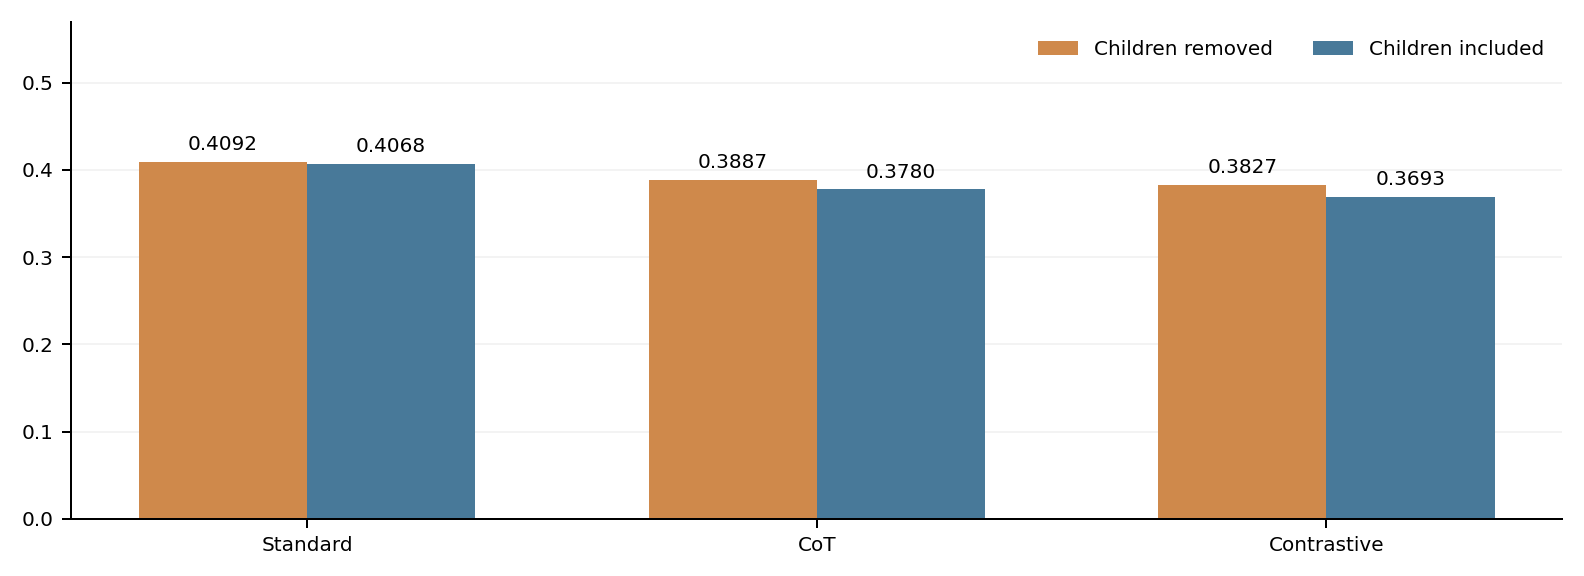
\includegraphics[width=\linewidth]{figures/child.png}
\caption{Llama seed 0 child-removal comparison on matched successful responses.}\label{figure:7.4}
\end{figure}

\begingroup
\begin{table}[!htbp]
\setlength{\tabcolsep}{3pt}
\renewcommand{\arraystretch}{1.18}
\fontsize{8.5}{10.5}\selectfont
\renewcommand{\thetable}{7.8}
\caption{Llama seed 0: paired child effects on F1: included minus removed.}\label{table:7.8}
\begin{tabular}{>{\raggedright\arraybackslash}p{\dimexpr 0.196078\linewidth-2\tabcolsep\relax}>{\raggedright\arraybackslash}p{\dimexpr 0.076253\linewidth-2\tabcolsep\relax}>{\raggedright\arraybackslash}p{\dimexpr 0.152505\linewidth-2\tabcolsep\relax}>{\raggedright\arraybackslash}p{\dimexpr 0.152505\linewidth-2\tabcolsep\relax}>{\raggedright\arraybackslash}p{\dimexpr 0.141612\linewidth-2\tabcolsep\relax}>{\raggedright\arraybackslash}p{\dimexpr 0.281046\linewidth-2\tabcolsep\relax}}
\toprule
\textbf{Style} & \textbf{n} & \textbf{Removed} & \textbf{Included} & \textbf{Effect} & \textbf{95\% interval} \\
\midrule
Standard & 451 & 0.4092 & 0.4068 & -0.0024 & [-0.0165, +0.0115] \\
CoT & 450 & 0.3887 & 0.3780 & -0.0108 & [-0.0256, +0.0038] \\
Contrastive & 448 & 0.3827 & 0.3693 & -0.0134 & [-0.0286, +0.0019] \\
\bottomrule
\end{tabular}
\end{table}
\endgroup


Figure~\ref{figure:7.4} and Table~\ref{table:7.8} show small negative point estimates in all three styles, but all three intervals include zero. These data establish neither a clear F1 benefit nor a clear F1 harm from including children. Under standard prompting, recall increases by 0.0176 and MRR by 0.0282, while precision falls by 0.0463 and hierarchical F1 by 0.0233. Narrower neighbours may help identify a class but also encourage additional unsupported specificity or a different broader hierarchy.


The planned cohort contains 451 entities. Completed pairs number 451 for standard, 450 for CoT, and 448 for contrastive: one child-removal CoT output and three eligible main contrastive outputs are incomplete. The matched denominators avoid treating those missing outputs as valid responses.


The experimental scope is a matched child-context intervention for Llama 3.1 8B Instruct at seed 0, across the three prompting styles and the 451 child-eligible entities. It measures the effect of the implemented child-removal treatment within this setting; cross-model comparisons are provided by the main nine-condition experiments.


\FloatBarrier

\section{Effects across taxonomy depth}

RQ3 and H2 concern whether graph benefit increases with depth. The maximum annotated-depth groups 4–5, 6–7, and 8+ contain 198, 465, and 337 entities before completion filtering. Table~\ref{table:7.9} reports paired F1 gains and actual denominators in each group.


\begingroup
\begin{table}[!htbp]
\setlength{\tabcolsep}{3pt}
\renewcommand{\arraystretch}{1.18}
\fontsize{8.5}{10.5}\selectfont
\renewcommand{\thetable}{7.9}
\caption{Mean paired F1 gains by maximum gold depth.}\label{table:7.9}
\begin{tabular}{>{\raggedright\arraybackslash}p{\dimexpr 0.313725\linewidth-2\tabcolsep\relax}>{\raggedright\arraybackslash}p{\dimexpr 0.228758\linewidth-2\tabcolsep\relax}>{\raggedright\arraybackslash}p{\dimexpr 0.228758\linewidth-2\tabcolsep\relax}>{\raggedright\arraybackslash}p{\dimexpr 0.228758\linewidth-2\tabcolsep\relax}}
\toprule
\textbf{Model/style} & \textbf{Depth 4–5} & \textbf{Depth 6–7} & \textbf{Depth 8+} \\
\midrule
Gemini Standard & +0.0872 (n=198) & +0.0608 (n=465) & +0.0503 (n=337) \\
Gemini CoT & +0.1362 (n=198) & +0.1254 (n=465) & +0.1351 (n=337) \\
Gemini Contrastive & +0.1473 (n=198) & +0.1190 (n=465) & +0.1492 (n=337) \\
Llama 0 Standard & +0.0890 (n=198) & +0.0551 (n=465) & +0.0481 (n=337) \\
Llama 0 CoT & +0.0623 (n=197) & +0.0567 (n=465) & +0.0469 (n=337) \\
Llama 0 Contrastive & +0.0688 (n=196) & +0.0513 (n=463) & +0.0701 (n=336) \\
Llama 42 Standard & +0.0822 (n=198) & +0.0313 (n=464) & +0.0514 (n=336) \\
Llama 42 CoT & +0.0801 (n=197) & +0.0438 (n=458) & +0.0322 (n=336) \\
Llama 42 Contrastive & +0.0888 (n=196) & +0.0525 (n=460) & +0.0586 (n=335) \\
Llama 123 Standard & +0.0670 (n=198) & +0.0371 (n=463) & +0.0432 (n=336) \\
Llama 123 CoT & +0.0819 (n=196) & +0.0448 (n=462) & +0.0315 (n=337) \\
Llama 123 Contrastive & +0.0861 (n=197) & +0.0668 (n=462) & +0.0638 (n=336) \\
\bottomrule
\end{tabular}
\end{table}
\endgroup


The analysis should be read as a profile of the observed cohort rather than a new universal depth law. The groups differ in vocabulary, description specificity, annotation length, and neighbourhood availability. Maximum gold depth also measures the shortest-root-distance convention of WiKC. It cannot be assumed equivalent to human-perceived conceptual difficulty.


Gains generally shrink with depth: the 4–5 stratum has the largest gain in 10 of the 12 rows. This pattern opposes H2, although it is not strictly monotonic in every row. Mean gold-list lengths are 10.28, 12.82, and 12.58 across the three strata. Shallow entities therefore have shorter gold lists, so a few parent labels can cover a larger fraction of G(e); the three-neighbour cap may therefore yield diminishing coverage at greater depth. This is a candidate explanation of the descriptive pattern, not a causal depth effect.


Future work should separate these factors using larger cohorts, continuous-depth models, and controls for the number of gold types and available neighbours. The present grouped results make the support and effects visible without fitting a causal trend to a small, heterogeneous sample.


\FloatBarrier

\section{Cases where graph context helps and hurts}

The examples below are selected from the new archives to illustrate positive and negative standard-prompt F1 changes. They are output comparisons, not independently validated semantic annotations or estimates of error frequency. Table~\ref{table:7.10} lists the descriptions and actual generated labels so that the effects can be inspected directly.


\begingroup
\begin{table}[!htbp]
\setlength{\tabcolsep}{3pt}
\renewcommand{\arraystretch}{1.18}
\fontsize{8.5}{10.5}\selectfont
\renewcommand{\thetable}{7.10}
\caption{Largest positive and negative standard F1 changes within each illustrated run.}\label{table:7.10}
\begin{tabular}{>{\raggedright\arraybackslash}p{\dimexpr 0.244009\linewidth-2\tabcolsep\relax}>{\raggedright\arraybackslash}p{\dimexpr 0.318083\linewidth-2\tabcolsep\relax}>{\raggedright\arraybackslash}p{\dimexpr 0.318083\linewidth-2\tabcolsep\relax}>{\raggedright\arraybackslash}p{\dimexpr 0.119826\linewidth-2\tabcolsep\relax}}
\toprule
\textbf{Entity and description} & \textbf{No-graph labels} & \textbf{Graph labels} & \textbf{F1} \\
\midrule
Gemini; Dave Matthews\newline fictional bartender in Family Affairs & fictional bartender; soap opera character; television character; fictional character; character; fictional entity; entity & fictional bartender; bartender; waiter; service worker; worker; person; person or organization; corporate body; object; entity & 0.1250 \ensuremath{\to} 0.8421\newline \ensuremath{\Delta} +0.7171 \\
Gemini; Alan Watts\newline English writer and lecturer (1915–1973) & writer; lecturer; professional; worker; person; person or organization; object; entity & writer; lecturer; author; speaker; intellectual; person; human; entity & 0.7059 \ensuremath{\to} 0.2353\newline \ensuremath{\Delta} -0.4706 \\
Llama 0; Left at London\newline American singer-songwriter and comedian & singer; songwriter; musician; performer; comedian; artist; person; individual; human; entity & media personality; celebrity; media professional; professional; person; person or organization; corporate body; object; entity & 0.1905 \ensuremath{\to} 0.9000\newline \ensuremath{\Delta} +0.7095 \\
Llama 0; Donald Bain\newline American writer & writer; author; creator; professional; worker; person; person or organization; corporate body; object; entity & writer; creator; human & 0.7059 \ensuremath{\to} 0.2000\newline \ensuremath{\Delta} -0.5059 \\
\bottomrule
\end{tabular}
\end{table}
\endgroup


For Dave Matthews, graph context recovers the annotated person-related chain while retaining fictional bartender; the larger F1 does not resolve whether that chain suits a fictional entity. Alan Watts loses broad gold labels despite retaining plausible occupations. For Left at London, the graph output shifts from occupations to the benchmark’s media-personality branch. Donald Bain’s graph output shrinks to three labels and loses coverage. These are exact-label disagreements, not independently established hallucinations.


Table~\ref{table:A.6} tests the possible demonstration effect by separating person entities (24.9\% of the cohort) from the rest and counting reproduction of the demonstration’s tail chain. Gains are not consistently concentrated in persons: Gemini’s standard gains are +0.0363 for persons and +0.0712 for other entities, while Llama seed 42 gives \ensuremath{-}0.0080 and +0.0668. Chain-frequency changes also vary by seed and style. These results weaken a simple person-imitation explanation; supported gold recovery and demonstration imitation cannot be separated without changing the demonstration.


\chapter{Discussion}

\FloatBarrier

\section{Main findings and contributions}

\subsection{Graph-aware prompting and label recovery}

RQ1 receives a consistent answer: graph-aware prompting improves all five main metrics in every model-by-style comparison, including all three Llama seeds. Each effect uses matched completed responses, so the two arms of a contrast contain the same entities. This supports the versioned prompting and evaluation design in C1 and C3, while the empty-child control shows why the effect should be described as a combination of structural evidence and instructions.


The experiment supports the use of a taxonomy as an inference-time evidence source. Parents can supply a semantic boundary and useful broader vocabulary. Siblings and children can describe nearby distinctions, while combined context allows the model to relate those distinctions to the description. The source of the improvement may include label availability, reduced uncertainty about the intended branch, and better ordering. The protocol does not isolate these mechanisms, so it would be premature to describe the gain as proof of graph reasoning in an internal cognitive sense.


Oracle selection is central to this interpretation. Removing the centre label from the context prevents direct copying of that field, but leaves an informative neighbourhood chosen using gold. The resulting gains justify testing retrieval: there is useful evidence available if the right structure can be located. They do not yet show that a model can locate it reliably or remain accurate when the supplied centre is wrong.


\subsection{Prompt style and model differences}

For RQ4, Gemini has higher paired F1 than every Llama seed in each of the nine conditions. Gemini’s highest graph F1 occurs with an explanation-bearing template, while the standard graph template leads the three combined-graph styles for Llama at every seed. These patterns support the matched empirical comparisons in C2, not a general architectural explanation. Gemini’s standard outputs already involve internal thinking, so asking for a visible explanation is not equivalent to turning reasoning on.


\subsection{Relation evidence and depth}

For RQ2, parent-only F1 exceeds sibling-only F1 throughout, which does not support H1. Combined context is not uniformly better than parent-only across Llama seeds. The seed-0 child intervention has slightly negative F1 point estimates, but every interval includes zero. A precision–recall trade-off is observed for standard prompting only. For RQ3, gains generally shrink with depth, with the largest gain in the shallowest stratum in 10 of 12 comparisons; H2 is not supported.


\subsection{Interpreting benchmark agreement}

The 265 descriptions containing the normalized centre label and the 735 descriptions without it both receive explicit analysis. Sixteen listed gold sets are not ancestor-closed, and 89 centres differ from Gmax(e). These checks explain why context selection, flat recovery, and hierarchical evaluation must remain distinct. Deterministic scores make the comparison reproducible, while semantic review is needed before interpreting every unmatched label as false.


\chapter{Conclusion}

This thesis investigated graph-aware prompting for entity typing using local WiKC taxonomy structure. The completed study compared standard, chain-of-thought, and contrastive prompting with and without combined graph evidence, added parent-, sibling-, and child-only conditions, and conducted a matched Llama seed-0 child-removal experiment. The supplied result archives contain 37,300 completed outputs from 37,353 planned entity–condition–run combinations. Incomplete results and attempts are retained and reported.


RQ1 receives a consistent answer within the experimental scope: graph-aware prompting improves F1, precision, recall, MRR, and depth-weighted nDCG across Gemini and all three Llama seeds. Paired F1 gains range from 0.0451 to 0.1348. The treatment supplies relevant oracle structure together with interpretation instructions, so it does not isolate evidence alone.


RQ2 shows that parent-only context outperforms sibling-only context on F1, contrary to H1. Including child context does not produce a general F1 gain in the matched seed-0 experiment. RQ3 shows gains generally shrinking with depth, contrary to H2. RQ4 shows higher Gemini F1 against each Llama seed in all nine matched condition comparisons, while the three Llama seeds expose variation in the relative strength of relation-only prompts.


The evaluation distinguishes several dimensions of performance. Recovering a maximum-depth gold label early is different from recovering an entire ancestor chain. Hierarchical closeness is different from explicitly listing a closed hierarchy. Exact benchmark agreement is different from complete semantic validity. These distinctions explain why the thesis presents several metrics, paired effects, distributions, and inspectable cases instead of one headline accuracy value.


The development process helped define that interpretation. Exploratory prompts were refined, an insufficiently useful taxonomy-extraction idea was abandoned, and generation controls were fixed for the final external-demonstration runs. Only the supplied new response archives contribute experimental scores; earlier outputs are excluded.


The empty-child control suggests a template contribution: point estimates range from about +0.005 to +0.024, with Gemini near +0.02 compared with its +0.0625 full-cohort standard gain. These different-cohort effects cannot be subtracted to isolate evidence, and the seed-123 interval includes zero. Gemini thinking-token increases also co-vary with graph gains, so structural evidence and additional computation are not isolated.


The conclusion is specific: oracle-selected local taxonomy evidence and its interpretation instructions form a useful inference-time prompt treatment for this ranked multi-label typing task. The study provides a reproducible basis for testing retrieved evidence, taxonomy quality, controlled noise, and independent semantic judgments.


\chapter{Limitations and future research}

\FloatBarrier

\section{Limitations and threats to validity}

The principal validity limitation is oracle context. The correct branch helps determine the supplied neighbourhood, so the structural treatment contains answer-related information. An autonomous system would need a candidate-selection stage that can fail. The current experiment is a diagnostic of evidence use, and its scores are not an estimate of end-to-end retrieval-and-typing performance.


Prompt development used earlier project examples, and all released entities remain in the final cohort. The external demonstration is outside that cohort, but this does not erase earlier prompt-selection exposure. A new entity set with frozen templates is needed before treating the findings as confirmatory.


The benchmark has automatic and graph-derived annotation choices. Gold ancestor chains may contain unusual categories, and descriptions can emphasize roles absent from the selected centre label. Exact matching rejects synonyms and extra valid labels. Ancestor augmentation partly accommodates structural proximity but introduces its own conventions, including roots, exact-gold disambiguation, and opaque unresolved predictions. No single reported metric is a complete semantic correctness measure.


Model comparability is bounded by the deployments. Gemini 3.8 Flash and the fixed Llama checkpoint differ in tokenizer, serving engine, context limit, training, and internal thinking. Temperature equality does not imply identical randomness. Model differences cannot be causally attributed to one architectural property.


Generation recovery conditions scores on validity, with different retry rates by condition. The Llama main runs have 9, 29, and 14 failed outputs, and the child intervention has one. Matched completion filtering and zero-for-failure sensitivity make those choices explicit; neither reproduces the distribution of unconstrained first calls. Three Llama seeds describe observed sampling variation, while Gemini has one run.


Bootstrap intervals quantify entity variation, not provider drift, demonstration choice, prompt-selection uncertainty, or all uncertainty in annotations. Many exploratory comparisons are reported without multiplicity correction. Relation-only lists also differ in length and availability, and the empty-child comparison changes more than the graph note. These points qualify mechanism claims without changing the observed direction of the primary contrasts.


The experiments cover WiKC context and the matched Llama child intervention. Comparisons with raw Wikidata, independent ancestor-path treatments, controlled noise, and quantitative taxonomy extraction remain directions for future research; the present data do not establish effects of graph quality or robustness.


\FloatBarrier

\section{Future research}

The immediate next step is to replace oracle centre selection with retrieval based only on the entity name and description. A useful evaluation should preserve the current oracle condition as an upper-information reference and compare it with retrieved and no-graph conditions on the same new entities. Retrieval precision, centre visibility, context quantity, and downstream typing should be measured separately. Descriptor-based candidate retrieval, as explored by \citet{ma2026}, provides one relevant direction.


A taxonomy-quality comparison could contrast WiKC with raw Wikidata. WiKC and the original Wikidata taxonomy should supply matched forms of context, with identical selection and label-resolution policies wherever possible. Structural differences can then be related to downstream changes. A higher score with one resource would still require checking whether the improvement arises from cleaner relations, a different label inventory, or easier access to gold ancestors.


Controlled noise would test the limits of the observed benefit. Parent replacement, sibling replacement, and irrelevant-child injection should be varied independently at known rates. Length-matched controls can distinguish structural misinformation from additional text alone. This would turn the general concern about distracting context into a specific robustness experiment for entity typing, rather than borrowing a conclusion from arithmetic reasoning research.


Neighbour selection deserves its own ablation. Sorting class identifiers is reproducible but not semantically optimized. Sampling several neighbour sets, selecting neighbours by description relevance, and varying the per-relation cap would test whether gains depend on arbitrary examples. A separate ancestor-path condition could examine whether broad-chain evidence improves recall differently from local alternatives.


Evaluation should combine deterministic scores with independent semantic review. New annotations can distinguish false types, valid synonyms, incomplete source gold, and role-versus-entity confusions. Reviewers should be blinded to prompting condition where practical, and agreement should be reported. Further seeds, repeated Gemini runs, and expanded first-call reliability analysis would complement the current accepted-response and retry results.


The abandoned extraction approach could return under stronger controls. Generated class proposals and links should be validated against independent evidence before being used for typing. Its contribution would be the downstream gain of validated inferred structure relative to fixed-resource and no-graph baselines. This would preserve the original ambition while separating extraction quality from classification ability.


These extensions follow directly from the current findings. Relevant structure is useful, relation families behave differently, and output metrics disagree in meaningful ways. The research challenge is now to retain that benefit when the graph evidence must be found, checked, and presented without access to the answer.


\appendix
\chapter{Detailed scores and diagnostics}

All results use only the four supplied response archives. Table~\ref{table:A.1} gives marginal completed-response means; contrasts in Tables A.4–A.6 use matched completed entities. The abbreviated condition codes are S = standard, C = CoT, X = contrastive; N = no graph, G = combined graph; P, B, and H = parent-, sibling-, and child-only standard prompts. L0, L42, and L123 identify Llama seeds. L0-S/C/X-R denotes child removal. Tables A.2 and A.3 report all nine main conditions and the three child-removal conditions.


\begingroup
\setlength{\tabcolsep}{3pt}
\renewcommand{\arraystretch}{1.18}
\fontsize{7.8}{9.5}\selectfont
\renewcommand{\thetable}{A.1}
\begin{longtable}{>{\raggedright\arraybackslash}p{\dimexpr 0.204793\linewidth-2\tabcolsep\relax}>{\raggedright\arraybackslash}p{\dimexpr 0.076253\linewidth-2\tabcolsep\relax}>{\raggedright\arraybackslash}p{\dimexpr 0.119826\linewidth-2\tabcolsep\relax}>{\raggedright\arraybackslash}p{\dimexpr 0.119826\linewidth-2\tabcolsep\relax}>{\raggedright\arraybackslash}p{\dimexpr 0.119826\linewidth-2\tabcolsep\relax}>{\raggedright\arraybackslash}p{\dimexpr 0.119826\linewidth-2\tabcolsep\relax}>{\raggedright\arraybackslash}p{\dimexpr 0.119826\linewidth-2\tabcolsep\relax}>{\raggedright\arraybackslash}p{\dimexpr 0.119826\linewidth-2\tabcolsep\relax}}
\caption{Completed-response scores and generated-label counts.}\label{table:A.1}\\
\toprule
\textbf{Run / condition} & \textbf{n} & \textbf{F1} & \textbf{P} & \textbf{R} & \textbf{MRR} & \textbf{nDCG} & \textbf{Labels} \\
\midrule
\endfirsthead
\multicolumn{8}{l}{\small Table A.1 (continued)}\\
\toprule
\textbf{Run / condition} & \textbf{n} & \textbf{F1} & \textbf{P} & \textbf{R} & \textbf{MRR} & \textbf{nDCG} & \textbf{Labels} \\
\midrule
\endhead
\midrule
\multicolumn{8}{r}{\small Continued on next page}\\
\endfoot
\bottomrule
\endlastfoot
Gem S-N & 1000 & 0.3888 & 0.4714 & 0.3503 & 0.2985 & 0.3188 & 8.3930 \\
Gem S-G & 1000 & 0.4513 & 0.5628 & 0.3968 & 0.4454 & 0.4611 & 8.0630 \\
Gem C-N & 1000 & 0.3389 & 0.4740 & 0.2782 & 0.2346 & 0.2709 & 6.6190 \\
Gem C-G & 1000 & 0.4696 & 0.6116 & 0.4000 & 0.5183 & 0.5028 & 7.4150 \\
Gem X-N & 1000 & 0.3330 & 0.4708 & 0.2704 & 0.2378 & 0.2686 & 6.4840 \\
Gem X-G & 1000 & 0.4678 & 0.6120 & 0.3969 & 0.5238 & 0.5028 & 7.3540 \\
Gem P & 1000 & 0.4302 & 0.5170 & 0.3891 & 0.4040 & 0.4218 & 8.5750 \\
Gem B & 1000 & 0.3958 & 0.4849 & 0.3533 & 0.4316 & 0.3853 & 8.3370 \\
Gem H & 1000 & 0.4160 & 0.5106 & 0.3727 & 0.3657 & 0.3573 & 8.1620 \\
L0 S-N & 1000 & 0.3391 & 0.3967 & 0.3325 & 0.1476 & 0.2339 & 10.7470 \\
L0 S-G & 1000 & 0.3986 & 0.4667 & 0.3819 & 0.1878 & 0.3692 & 9.6570 \\
L0 C-N & 999 & 0.3214 & 0.3658 & 0.3158 & 0.1693 & 0.2297 & 10.0511 \\
L0 C-G & 1000 & 0.3759 & 0.4258 & 0.3720 & 0.1977 & 0.3554 & 10.1680 \\
L0 X-N & 999 & 0.3055 & 0.3540 & 0.2961 & 0.1654 & 0.2161 & 9.7107 \\
L0 X-G & 996 & 0.3668 & 0.4389 & 0.3471 & 0.2088 & 0.3449 & 9.2570 \\
L0 P & 998 & 0.4029 & 0.4752 & 0.3822 & 0.1773 & 0.3707 & 9.6743 \\
L0 B & 999 & 0.3417 & 0.3965 & 0.3303 & 0.1733 & 0.2564 & 9.8569 \\
L0 H & 1000 & 0.3510 & 0.4117 & 0.3415 & 0.1512 & 0.2357 & 10.3170 \\
L42 S-N & 1000 & 0.3482 & 0.3985 & 0.3451 & 0.1447 & 0.2371 & 10.8750 \\
L42 S-G & 998 & 0.3962 & 0.4675 & 0.3786 & 0.1895 & 0.3755 & 9.8186 \\
L42 C-N & 999 & 0.3245 & 0.3687 & 0.3179 & 0.1693 & 0.2271 & 10.0611 \\
L42 C-G & 992 & 0.3715 & 0.4297 & 0.3608 & 0.2131 & 0.3585 & 9.8942 \\
L42 X-N & 996 & 0.3117 & 0.3596 & 0.2997 & 0.1698 & 0.2210 & 9.6797 \\
L42 X-G & 995 & 0.3740 & 0.4400 & 0.3578 & 0.2023 & 0.3491 & 9.6432 \\
L42 P & 999 & 0.4076 & 0.4661 & 0.3942 & 0.1849 & 0.3786 & 9.8729 \\
L42 B & 994 & 0.3639 & 0.4189 & 0.3519 & 0.1748 & 0.2651 & 9.8592 \\
L42 H & 998 & 0.3688 & 0.4248 & 0.3595 & 0.1560 & 0.2431 & 10.0080 \\
L123 S-N & 1000 & 0.3461 & 0.3940 & 0.3406 & 0.1544 & 0.2336 & 10.8500 \\
L123 S-G & 997 & 0.3910 & 0.4613 & 0.3696 & 0.1843 & 0.3635 & 9.6369 \\
L123 C-N & 996 & 0.3322 & 0.3792 & 0.3238 & 0.1730 & 0.2356 & 9.7129 \\
L123 C-G & 999 & 0.3794 & 0.4330 & 0.3714 & 0.2053 & 0.3548 & 10.0591 \\
L123 X-N & 996 & 0.3024 & 0.3467 & 0.2918 & 0.1701 & 0.2210 & 9.8072 \\
L123 X-G & 999 & 0.3717 & 0.4315 & 0.3571 & 0.1948 & 0.3493 & 9.8188 \\
L123 P & 1000 & 0.3674 & 0.4704 & 0.3412 & 0.1992 & 0.3683 & 8.4710 \\
L123 B & 1000 & 0.3476 & 0.4087 & 0.3374 & 0.1664 & 0.2510 & 9.8570 \\
L123 H & 999 & 0.3372 & 0.4053 & 0.3265 & 0.1627 & 0.2319 & 9.2823 \\
L0 S-R & 451 & 0.4092 & 0.5188 & 0.3767 & 0.1864 & 0.3768 & 8.4568 \\
L0 C-R & 450 & 0.3887 & 0.4484 & 0.3818 & 0.2335 & 0.3689 & 9.6622 \\
L0 X-R & 451 & 0.3831 & 0.4560 & 0.3621 & 0.2343 & 0.3548 & 8.9601 \\
\end{longtable}
\endgroup


Table~\ref{table:A.2a} reports pooled micro-F1, strict set accuracy, mean ancestor-augmented F1, and mean hierarchy consistency. Consistency averages the fraction of resolved predicted graph nodes whose ancestors already occur in the output; its eligible entity count excludes outputs with no resolved graph nodes. Loose macro-F1 is the harmonic mean of mean precision and mean recall and differs from mean entity F1.


\begingroup
\setlength{\tabcolsep}{3pt}
\renewcommand{\arraystretch}{1.18}
\fontsize{7.8}{9.5}\selectfont
\renewcommand{\thetable}{A.2a}
\begin{longtable}{>{\raggedright\arraybackslash}p{\dimexpr 0.215686\linewidth-2\tabcolsep\relax}>{\raggedright\arraybackslash}p{\dimexpr 0.130719\linewidth-2\tabcolsep\relax}>{\raggedright\arraybackslash}p{\dimexpr 0.130719\linewidth-2\tabcolsep\relax}>{\raggedright\arraybackslash}p{\dimexpr 0.130719\linewidth-2\tabcolsep\relax}>{\raggedright\arraybackslash}p{\dimexpr 0.130719\linewidth-2\tabcolsep\relax}>{\raggedright\arraybackslash}p{\dimexpr 0.130719\linewidth-2\tabcolsep\relax}>{\raggedright\arraybackslash}p{\dimexpr 0.130719\linewidth-2\tabcolsep\relax}}
\caption{Set and hierarchy diagnostics. Rates are proportions.}\label{table:A.2a}\label{table:A.2}\\
\toprule
\textbf{Run / condition} & \textbf{Micro F1} & \textbf{Loose F1} & \textbf{Strict acc.} & \textbf{Hier. F1} & \textbf{Consist.} & \textbf{Eligible n} \\
\midrule
\endfirsthead
\multicolumn{7}{l}{\small Table A.2a (continued)}\\
\toprule
\textbf{Run / condition} & \textbf{Micro F1} & \textbf{Loose F1} & \textbf{Strict acc.} & \textbf{Hier. F1} & \textbf{Consist.} & \textbf{Eligible n} \\
\midrule
\endhead
\midrule
\multicolumn{7}{r}{\small Continued on next page}\\
\endfoot
\bottomrule
\endlastfoot
Gem S-N & 0.3831 & 0.4019 & 0.0010 & 0.6985 & 0.3282 & 1000 \\
Gem S-G & 0.4443 & 0.4655 & 0.0010 & 0.7963 & 0.2380 & 999 \\
Gem C-N & 0.3323 & 0.3506 & 0.0010 & 0.6720 & 0.3675 & 997 \\
Gem C-G & 0.4595 & 0.4837 & 0.0010 & 0.8302 & 0.2455 & 999 \\
Gem X-N & 0.3248 & 0.3435 & 0.0000 & 0.6815 & 0.3559 & 998 \\
Gem X-G & 0.4567 & 0.4815 & 0.0010 & 0.8318 & 0.2455 & 999 \\
Gem P & 0.4244 & 0.4440 & 0.0010 & 0.7634 & 0.2452 & 998 \\
Gem B & 0.3905 & 0.4088 & 0.0000 & 0.7405 & 0.2585 & 999 \\
Gem H & 0.4098 & 0.4309 & 0.0010 & 0.7259 & 0.3318 & 997 \\
L0 S-N & 0.3234 & 0.3618 & 0.0000 & 0.5668 & 0.5479 & 1000 \\
L0 S-G & 0.3838 & 0.4201 & 0.0000 & 0.7214 & 0.4298 & 999 \\
L0 C-N & 0.3143 & 0.3390 & 0.0000 & 0.5608 & 0.5014 & 992 \\
L0 C-G & 0.3675 & 0.3971 & 0.0000 & 0.7081 & 0.3733 & 998 \\
L0 X-N & 0.2978 & 0.3225 & 0.0000 & 0.5617 & 0.4829 & 993 \\
L0 X-G & 0.3569 & 0.3876 & 0.0000 & 0.7284 & 0.3378 & 995 \\
L0 P & 0.3880 & 0.4237 & 0.0010 & 0.7145 & 0.4253 & 998 \\
L0 B & 0.3285 & 0.3604 & 0.0000 & 0.6015 & 0.4718 & 997 \\
L0 H & 0.3316 & 0.3733 & 0.0000 & 0.5807 & 0.5292 & 999 \\
L42 S-N & 0.3287 & 0.3699 & 0.0000 & 0.5614 & 0.5619 & 998 \\
L42 S-G & 0.3830 & 0.4184 & 0.0000 & 0.7260 & 0.3992 & 997 \\
L42 C-N & 0.3169 & 0.3414 & 0.0010 & 0.5572 & 0.5275 & 996 \\
L42 C-G & 0.3639 & 0.3923 & 0.0000 & 0.7135 & 0.3466 & 990 \\
L42 X-N & 0.3047 & 0.3269 & 0.0000 & 0.5702 & 0.4765 & 988 \\
L42 X-G & 0.3633 & 0.3947 & 0.0000 & 0.7241 & 0.3451 & 993 \\
L42 P & 0.3937 & 0.4272 & 0.0010 & 0.7129 & 0.4491 & 999 \\
L42 B & 0.3497 & 0.3825 & 0.0010 & 0.6029 & 0.5132 & 993 \\
L42 H & 0.3541 & 0.3894 & 0.0000 & 0.5918 & 0.5744 & 998 \\
L123 S-N & 0.3271 & 0.3653 & 0.0000 & 0.5558 & 0.5690 & 1000 \\
L123 S-G & 0.3766 & 0.4104 & 0.0000 & 0.7222 & 0.3997 & 996 \\
L123 C-N & 0.3230 & 0.3493 & 0.0000 & 0.5740 & 0.5015 & 989 \\
L123 C-G & 0.3709 & 0.3998 & 0.0010 & 0.7089 & 0.3719 & 998 \\
L123 X-N & 0.2942 & 0.3169 & 0.0000 & 0.5702 & 0.4748 & 994 \\
L123 X-G & 0.3611 & 0.3908 & 0.0000 & 0.7198 & 0.3419 & 999 \\
L123 P & 0.3662 & 0.3955 & 0.0000 & 0.7253 & 0.3581 & 988 \\
L123 B & 0.3358 & 0.3696 & 0.0010 & 0.5960 & 0.5190 & 998 \\
L123 H & 0.3338 & 0.3617 & 0.0010 & 0.5788 & 0.5390 & 968 \\
L0 S-R & 0.3978 & 0.4365 & 0.0000 & 0.7534 & 0.4001 & 451 \\
L0 C-R & 0.3819 & 0.4124 & 0.0000 & 0.7239 & 0.3783 & 450 \\
L0 X-R & 0.3749 & 0.4037 & 0.0000 & 0.7360 & 0.3332 & 451 \\
\end{longtable}
\endgroup


Table~\ref{table:A.2b} reports the first matching rank for any maximum-depth gold label. Rank bins sum to n, and hit rate equals one minus the miss proportion.


\begingroup
\setlength{\tabcolsep}{3pt}
\renewcommand{\arraystretch}{1.18}
\fontsize{7.8}{9.5}\selectfont
\renewcommand{\thetable}{A.2b}
\begin{longtable}{>{\raggedright\arraybackslash}p{\dimexpr 0.215686\linewidth-2\tabcolsep\relax}>{\raggedright\arraybackslash}p{\dimexpr 0.130719\linewidth-2\tabcolsep\relax}>{\raggedright\arraybackslash}p{\dimexpr 0.130719\linewidth-2\tabcolsep\relax}>{\raggedright\arraybackslash}p{\dimexpr 0.130719\linewidth-2\tabcolsep\relax}>{\raggedright\arraybackslash}p{\dimexpr 0.130719\linewidth-2\tabcolsep\relax}>{\raggedright\arraybackslash}p{\dimexpr 0.130719\linewidth-2\tabcolsep\relax}>{\raggedright\arraybackslash}p{\dimexpr 0.130719\linewidth-2\tabcolsep\relax}}
\caption{Maximum-depth hit rate and rank-bin counts.}\label{table:A.2b}\\
\toprule
\textbf{Run / condition} & \textbf{n} & \textbf{Hit rate} & \textbf{Rank 1} & \textbf{Rank 2} & \textbf{Rank 3+} & \textbf{Miss} \\
\midrule
\endfirsthead
\multicolumn{7}{l}{\small Table A.2b (continued)}\\
\toprule
\textbf{Run / condition} & \textbf{n} & \textbf{Hit rate} & \textbf{Rank 1} & \textbf{Rank 2} & \textbf{Rank 3+} & \textbf{Miss} \\
\midrule
\endhead
\midrule
\multicolumn{7}{r}{\small Continued on next page}\\
\endfoot
\bottomrule
\endlastfoot
Gem S-N & 1000 & 0.4200 & 218 & 111 & 91 & 580 \\
Gem S-G & 1000 & 0.5930 & 348 & 129 & 116 & 407 \\
Gem C-N & 1000 & 0.3000 & 186 & 72 & 42 & 700 \\
Gem C-G & 1000 & 0.6290 & 439 & 111 & 79 & 371 \\
Gem X-N & 1000 & 0.3060 & 188 & 74 & 44 & 694 \\
Gem X-G & 1000 & 0.6300 & 449 & 105 & 76 & 370 \\
Gem P & 1000 & 0.5680 & 303 & 130 & 135 & 432 \\
Gem B & 1000 & 0.5760 & 334 & 137 & 105 & 424 \\
Gem H & 1000 & 0.4850 & 285 & 112 & 88 & 515 \\
L0 S-N & 1000 & 0.1850 & 124 & 32 & 29 & 815 \\
L0 S-G & 1000 & 0.2610 & 140 & 59 & 62 & 739 \\
L0 C-N & 999 & 0.2112 & 140 & 46 & 25 & 788 \\
L0 C-G & 1000 & 0.2970 & 136 & 77 & 84 & 703 \\
L0 X-N & 999 & 0.2112 & 137 & 37 & 37 & 788 \\
L0 X-G & 996 & 0.2972 & 151 & 79 & 66 & 700 \\
L0 P & 998 & 0.2405 & 133 & 61 & 46 & 758 \\
L0 B & 999 & 0.2062 & 153 & 25 & 28 & 793 \\
L0 H & 1000 & 0.2010 & 120 & 43 & 38 & 799 \\
L42 S-N & 1000 & 0.1820 & 120 & 36 & 26 & 818 \\
L42 S-G & 998 & 0.2725 & 137 & 66 & 69 & 726 \\
L42 C-N & 999 & 0.2102 & 142 & 36 & 32 & 789 \\
L42 C-G & 992 & 0.3054 & 155 & 67 & 81 & 689 \\
L42 X-N & 996 & 0.2309 & 128 & 60 & 42 & 766 \\
L42 X-G & 995 & 0.3035 & 139 & 75 & 88 & 693 \\
L42 P & 999 & 0.2492 & 139 & 67 & 43 & 750 \\
L42 B & 994 & 0.2113 & 149 & 35 & 26 & 784 \\
L42 H & 998 & 0.2134 & 120 & 48 & 45 & 785 \\
L123 S-N & 1000 & 0.1820 & 136 & 28 & 18 & 818 \\
L123 S-G & 997 & 0.2568 & 135 & 67 & 54 & 741 \\
L123 C-N & 996 & 0.2189 & 141 & 46 & 31 & 778 \\
L123 C-G & 999 & 0.3013 & 147 & 72 & 82 & 698 \\
L123 X-N & 996 & 0.2269 & 132 & 54 & 40 & 770 \\
L123 X-G & 999 & 0.2993 & 131 & 75 & 93 & 700 \\
L123 P & 1000 & 0.2620 & 152 & 74 & 36 & 738 \\
L123 B & 1000 & 0.2040 & 141 & 35 & 28 & 796 \\
L123 H & 999 & 0.2092 & 132 & 44 & 33 & 790 \\
L0 S-R & 451 & 0.2749 & 56 & 38 & 30 & 327 \\
L0 C-R & 450 & 0.3400 & 74 & 37 & 42 & 297 \\
L0 X-R & 451 & 0.3459 & 71 & 48 & 37 & 295 \\
\end{longtable}
\endgroup


Table~\ref{table:A.3a} counts unique normalized predictions, pooled over completed entities. E = exact gold, Br = broader, Na = narrower, Si = sibling, O = other connected taxonomy label, U = unresolved or unavailable distance. Classification uses the precedence in Section 6.3. Because gold includes broad ancestors such as entity, many incorrect graph labels fall into Na; this need not mean they are narrower than the centre. Table~\ref{table:A.3b} separates U into outside-label-inventory (Out), ambiguous (Amb), label without graph node (No node), and disconnected (Disc). A label missing from the label index is operationally outside the supplied inventory, not necessarily semantically invalid.


\begingroup
\setlength{\tabcolsep}{3pt}
\renewcommand{\arraystretch}{1.18}
\fontsize{7.8}{9.5}\selectfont
\renewcommand{\thetable}{A.3a}
\begin{longtable}{>{\raggedright\arraybackslash}p{\dimexpr 0.215686\linewidth-2\tabcolsep\relax}>{\raggedright\arraybackslash}p{\dimexpr 0.130719\linewidth-2\tabcolsep\relax}>{\raggedright\arraybackslash}p{\dimexpr 0.108932\linewidth-2\tabcolsep\relax}>{\raggedright\arraybackslash}p{\dimexpr 0.108932\linewidth-2\tabcolsep\relax}>{\raggedright\arraybackslash}p{\dimexpr 0.108932\linewidth-2\tabcolsep\relax}>{\raggedright\arraybackslash}p{\dimexpr 0.108932\linewidth-2\tabcolsep\relax}>{\raggedright\arraybackslash}p{\dimexpr 0.108932\linewidth-2\tabcolsep\relax}>{\raggedright\arraybackslash}p{\dimexpr 0.108932\linewidth-2\tabcolsep\relax}}
\caption{Prediction-level error directions.}\label{table:A.3a}\label{table:A.3}\\
\toprule
\textbf{Run / condition} & \textbf{Total} & \textbf{E} & \textbf{Br} & \textbf{Na} & \textbf{Si} & \textbf{O} & \textbf{U} \\
\midrule
\endfirsthead
\multicolumn{8}{l}{\small Table A.3a (continued)}\\
\toprule
\textbf{Run / condition} & \textbf{Total} & \textbf{E} & \textbf{Br} & \textbf{Na} & \textbf{Si} & \textbf{O} & \textbf{U} \\
\midrule
\endhead
\midrule
\multicolumn{8}{r}{\small Continued on next page}\\
\endfoot
\bottomrule
\endlastfoot
Gem S-N & 8393 & 3952 & 1 & 1066 & 0 & 0 & 3374 \\
Gem S-G & 8063 & 4510 & 3 & 893 & 0 & 0 & 2657 \\
Gem C-N & 6619 & 3133 & 0 & 772 & 0 & 0 & 2714 \\
Gem C-G & 7415 & 4515 & 4 & 660 & 0 & 0 & 2236 \\
Gem X-N & 6484 & 3040 & 0 & 763 & 0 & 0 & 2681 \\
Gem X-G & 7354 & 4474 & 4 & 632 & 0 & 0 & 2244 \\
Gem P & 8575 & 4416 & 1 & 990 & 0 & 0 & 3168 \\
Gem B & 8337 & 4017 & 0 & 1025 & 0 & 0 & 3295 \\
Gem H & 8162 & 4180 & 0 & 977 & 0 & 0 & 3005 \\
L0 S-N & 10613 & 3695 & 0 & 1150 & 0 & 0 & 5768 \\
L0 S-G & 9615 & 4194 & 4 & 978 & 0 & 0 & 4439 \\
L0 C-N & 9985 & 3490 & 0 & 1007 & 0 & 0 & 5488 \\
L0 C-G & 10105 & 4106 & 4 & 1067 & 0 & 0 & 4928 \\
L0 X-N & 9684 & 3263 & 0 & 931 & 0 & 0 & 5490 \\
L0 X-G & 9183 & 3814 & 4 & 1029 & 0 & 0 & 4336 \\
L0 P & 9429 & 4199 & 4 & 828 & 0 & 0 & 4398 \\
L0 B & 9741 & 3608 & 0 & 1082 & 0 & 0 & 5051 \\
L0 H & 10190 & 3719 & 0 & 1178 & 0 & 0 & 5293 \\
L42 S-N & 10689 & 3768 & 0 & 1122 & 0 & 0 & 5799 \\
L42 S-G & 9701 & 4196 & 4 & 880 & 0 & 0 & 4621 \\
L42 C-N & 10007 & 3521 & 0 & 936 & 0 & 0 & 5550 \\
L42 C-G & 9764 & 3985 & 3 & 1090 & 0 & 0 & 4686 \\
L42 X-N & 9606 & 3321 & 0 & 952 & 0 & 0 & 5333 \\
L42 X-G & 9541 & 3947 & 4 & 1073 & 0 & 0 & 4517 \\
L42 P & 9822 & 4341 & 4 & 841 & 0 & 0 & 4636 \\
L42 B & 9770 & 3836 & 0 & 1041 & 0 & 0 & 4893 \\
L42 H & 9879 & 3909 & 0 & 1118 & 0 & 0 & 4852 \\
L123 S-N & 10724 & 3755 & 0 & 1138 & 0 & 0 & 5831 \\
L123 S-G & 9551 & 4096 & 3 & 868 & 0 & 0 & 4584 \\
L123 C-N & 9654 & 3530 & 0 & 925 & 0 & 0 & 5199 \\
L123 C-G & 9992 & 4121 & 3 & 1047 & 0 & 0 & 4821 \\
L123 X-N & 9751 & 3225 & 0 & 952 & 0 & 0 & 5574 \\
L123 X-G & 9766 & 3971 & 4 & 1092 & 0 & 0 & 4699 \\
L123 P & 8460 & 3790 & 4 & 725 & 0 & 0 & 3941 \\
L123 B & 9825 & 3704 & 0 & 1060 & 0 & 0 & 5061 \\
L123 H & 9208 & 3577 & 0 & 1056 & 0 & 0 & 4575 \\
L0 S-R & 3762 & 1812 & 2 & 293 & 0 & 0 & 1655 \\
L0 C-R & 4325 & 1845 & 2 & 361 & 0 & 0 & 2117 \\
L0 X-R & 4020 & 1756 & 2 & 377 & 0 & 0 & 1885 \\
\end{longtable}
\endgroup


Finite-distance means in Table~\ref{table:A.3b} pool mapped incorrect labels (Err n). Entity means first average finite errors within each eligible entity, then average over those entities (Ent n). Outputs without a finite-distance error are excluded from that entity mean. Exact matches are excluded from both distance summaries. Distances use the nearest listed gold class, which can be a broad ancestor.


\begingroup
\setlength{\tabcolsep}{3pt}
\renewcommand{\arraystretch}{1.18}
\fontsize{7.8}{9.5}\selectfont
\renewcommand{\thetable}{A.3b}
\begin{longtable}{>{\raggedright\arraybackslash}p{\dimexpr 0.215686\linewidth-2\tabcolsep\relax}>{\raggedright\arraybackslash}p{\dimexpr 0.087146\linewidth-2\tabcolsep\relax}>{\raggedright\arraybackslash}p{\dimexpr 0.087146\linewidth-2\tabcolsep\relax}>{\raggedright\arraybackslash}p{\dimexpr 0.098039\linewidth-2\tabcolsep\relax}>{\raggedright\arraybackslash}p{\dimexpr 0.076253\linewidth-2\tabcolsep\relax}>{\raggedright\arraybackslash}p{\dimexpr 0.108932\linewidth-2\tabcolsep\relax}>{\raggedright\arraybackslash}p{\dimexpr 0.108932\linewidth-2\tabcolsep\relax}>{\raggedright\arraybackslash}p{\dimexpr 0.098039\linewidth-2\tabcolsep\relax}>{\raggedright\arraybackslash}p{\dimexpr 0.119826\linewidth-2\tabcolsep\relax}}
\caption{Unavailable-distance counts and finite error distances.}\label{table:A.3b}\\
\toprule
\textbf{Run / condition} & \textbf{Out} & \textbf{Amb} & \textbf{No node} & \textbf{Disc} & \textbf{Err n} & \textbf{Pooled mean} & \textbf{Ent n} & \textbf{Entity mean} \\
\midrule
\endfirsthead
\multicolumn{9}{l}{\small Table A.3b (continued)}\\
\toprule
\textbf{Run / condition} & \textbf{Out} & \textbf{Amb} & \textbf{No node} & \textbf{Disc} & \textbf{Err n} & \textbf{Pooled mean} & \textbf{Ent n} & \textbf{Entity mean} \\
\midrule
\endhead
\midrule
\multicolumn{9}{r}{\small Continued on next page}\\
\endfoot
\bottomrule
\endlastfoot
Gem S-N & 1153 & 1106 & 1115 & 0 & 1067 & 1.7648 & 637 & 1.6407 \\
Gem S-G & 740 & 880 & 1037 & 0 & 896 & 1.6741 & 580 & 1.5624 \\
Gem C-N & 896 & 961 & 857 & 0 & 772 & 1.6956 & 527 & 1.6135 \\
Gem C-G & 608 & 817 & 811 & 0 & 664 & 1.5904 & 473 & 1.4943 \\
Gem X-N & 908 & 933 & 840 & 0 & 763 & 1.7444 & 537 & 1.6488 \\
Gem X-G & 640 & 828 & 776 & 0 & 636 & 1.5928 & 461 & 1.5318 \\
Gem P & 1023 & 1006 & 1139 & 0 & 991 & 1.7497 & 593 & 1.6337 \\
Gem B & 1087 & 1045 & 1163 & 0 & 1025 & 1.7737 & 627 & 1.6496 \\
Gem H & 925 & 1056 & 1024 & 0 & 977 & 1.7410 & 609 & 1.6304 \\
L0 S-N & 2706 & 2007 & 1055 & 0 & 1150 & 1.7843 & 661 & 1.7093 \\
L0 S-G & 2045 & 1509 & 885 & 0 & 982 & 1.7536 & 644 & 1.6944 \\
L0 C-N & 2464 & 1903 & 1121 & 0 & 1007 & 1.7855 & 611 & 1.7361 \\
L0 C-G & 2321 & 1631 & 976 & 0 & 1071 & 1.5808 & 612 & 1.5946 \\
L0 X-N & 2503 & 1848 & 1139 & 0 & 931 & 1.8346 & 592 & 1.7445 \\
L0 X-G & 2126 & 1422 & 788 & 0 & 1033 & 1.5189 & 597 & 1.5532 \\
L0 P & 1913 & 1588 & 897 & 0 & 832 & 1.8053 & 563 & 1.7692 \\
L0 B & 2142 & 1852 & 1057 & 0 & 1082 & 1.8179 & 646 & 1.7558 \\
L0 H & 2457 & 1903 & 933 & 0 & 1178 & 1.7971 & 679 & 1.7504 \\
L42 S-N & 2715 & 1952 & 1132 & 0 & 1122 & 1.8191 & 679 & 1.7605 \\
L42 S-G & 2262 & 1472 & 887 & 0 & 884 & 1.6742 & 574 & 1.6406 \\
L42 C-N & 2519 & 1808 & 1223 & 0 & 936 & 1.8686 & 625 & 1.8031 \\
L42 C-G & 2137 & 1572 & 977 & 0 & 1093 & 1.5782 & 609 & 1.5997 \\
L42 X-N & 2362 & 1745 & 1226 & 0 & 952 & 1.7826 & 597 & 1.6772 \\
L42 X-G & 2126 & 1518 & 873 & 0 & 1077 & 1.5664 & 608 & 1.5841 \\
L42 P & 2099 & 1580 & 957 & 0 & 845 & 1.8639 & 576 & 1.8191 \\
L42 B & 1967 & 1890 & 1036 & 0 & 1041 & 1.7944 & 658 & 1.7876 \\
L42 H & 2051 & 1874 & 927 & 0 & 1118 & 1.7710 & 652 & 1.7198 \\
L123 S-N & 2445 & 2150 & 1236 & 0 & 1138 & 1.8743 & 659 & 1.8197 \\
L123 S-G & 2264 & 1428 & 892 & 0 & 871 & 1.7371 & 562 & 1.7181 \\
L123 C-N & 2298 & 1855 & 1046 & 0 & 925 & 1.7978 & 598 & 1.7773 \\
L123 C-G & 2187 & 1705 & 929 & 0 & 1050 & 1.6543 & 632 & 1.6721 \\
L123 X-N & 2565 & 1795 & 1214 & 0 & 952 & 1.8067 & 615 & 1.7493 \\
L123 X-G & 2109 & 1662 & 928 & 0 & 1096 & 1.5776 & 615 & 1.5477 \\
L123 P & 1776 & 1343 & 822 & 0 & 729 & 1.8999 & 516 & 1.8460 \\
L123 B & 2101 & 1958 & 1002 & 0 & 1060 & 1.7509 & 649 & 1.6811 \\
L123 H & 1960 & 1757 & 858 & 0 & 1056 & 1.8267 & 621 & 1.7678 \\
L0 S-R & 757 & 560 & 338 & 0 & 295 & 2.0102 & 209 & 1.9820 \\
L0 C-R & 906 & 747 & 464 & 0 & 363 & 1.7713 & 243 & 1.8038 \\
L0 X-R & 875 & 627 & 383 & 0 & 379 & 1.6992 & 243 & 1.7481 \\
\end{longtable}
\endgroup


Table~\ref{table:A.4} gives paired F1 effects and entity-bootstrap intervals for all primary model/style comparisons. H/T/D count helped/tied/harmed entities; ties use absolute difference at most 10\textsuperscript{-12}. The no-graph and graph means use the same completed entities in each row.


\begingroup
\setlength{\tabcolsep}{3pt}
\renewcommand{\arraystretch}{1.18}
\fontsize{7.8}{9.5}\selectfont
\renewcommand{\thetable}{A.4}
\begin{longtable}{>{\raggedright\arraybackslash}p{\dimexpr 0.226580\linewidth-2\tabcolsep\relax}>{\raggedright\arraybackslash}p{\dimexpr 0.065359\linewidth-2\tabcolsep\relax}>{\raggedright\arraybackslash}p{\dimexpr 0.104575\linewidth-2\tabcolsep\relax}>{\raggedright\arraybackslash}p{\dimexpr 0.104575\linewidth-2\tabcolsep\relax}>{\raggedright\arraybackslash}p{\dimexpr 0.104575\linewidth-2\tabcolsep\relax}>{\raggedright\arraybackslash}p{\dimexpr 0.239651\linewidth-2\tabcolsep\relax}>{\raggedright\arraybackslash}p{\dimexpr 0.154684\linewidth-2\tabcolsep\relax}}
\caption{Primary paired F1 contrasts and change counts.}\label{table:A.4}\\
\toprule
\textbf{Run / style} & \textbf{n} & \textbf{No graph} & \textbf{Graph} & \textbf{Gain} & \textbf{95\% interval} & \textbf{H / T / D} \\
\midrule
\endfirsthead
\multicolumn{7}{l}{\small Table A.4 (continued)}\\
\toprule
\textbf{Run / style} & \textbf{n} & \textbf{No graph} & \textbf{Graph} & \textbf{Gain} & \textbf{95\% interval} & \textbf{H / T / D} \\
\midrule
\endhead
\midrule
\multicolumn{7}{r}{\small Continued on next page}\\
\endfoot
\bottomrule
\endlastfoot
Gemini Standard & 1000 & 0.3888 & 0.4513 & +0.0625 & [+0.0539, +0.0711] & 661/87/252 \\
Gemini CoT & 1000 & 0.3389 & 0.4696 & +0.1308 & [+0.1215, +0.1399] & 788/56/156 \\
Gemini Contrastive & 1000 & 0.3330 & 0.4678 & +0.1348 & [+0.1258, +0.1438] & 795/63/142 \\
Llama 0 Standard & 1000 & 0.3391 & 0.3986 & +0.0594 & [+0.0493, +0.0691] & 661/27/312 \\
Llama 0 CoT & 999 & 0.3214 & 0.3759 & +0.0545 & [+0.0443, +0.0646] & 612/34/353 \\
Llama 0 Contrastive & 995 & 0.3057 & 0.3668 & +0.0611 & [+0.0509, +0.0712] & 645/41/309 \\
Llama 42 Standard & 998 & 0.3481 & 0.3962 & +0.0482 & [+0.0378, +0.0583] & 618/39/341 \\
Llama 42 CoT & 991 & 0.3245 & 0.3716 & +0.0471 & [+0.0369, +0.0570] & 612/34/345 \\
Llama 42 Contrastive & 991 & 0.3118 & 0.3735 & +0.0617 & [+0.0512, +0.0725] & 623/39/329 \\
Llama 123 Standard & 997 & 0.3459 & 0.3910 & +0.0451 & [+0.0351, +0.0553] & 615/41/341 \\
Llama 123 CoT & 995 & 0.3318 & 0.3794 & +0.0476 & [+0.0367, +0.0581] & 616/37/342 \\
Llama 123 Contrastive & 995 & 0.3024 & 0.3720 & +0.0696 & [+0.0598, +0.0793] & 644/48/303 \\
\end{longtable}
\endgroup


Table~\ref{table:A.5} reports Gemini minus each Llama seed, with 2,000 entity-bootstrap resamples. Condition rows compare F1 scores on shared completed entities. Gain rows compare graph-minus-no-graph F1 effects on the intersection of all four required outputs. These intervals condition on the recorded model runs, rather than resampling model seeds.


\begingroup
\setlength{\tabcolsep}{3pt}
\renewcommand{\arraystretch}{1.18}
\fontsize{7.8}{9.5}\selectfont
\renewcommand{\thetable}{A.5}
\begin{longtable}{>{\raggedright\arraybackslash}p{\dimexpr 0.433551\linewidth-2\tabcolsep\relax}>{\raggedright\arraybackslash}p{\dimexpr 0.087146\linewidth-2\tabcolsep\relax}>{\raggedright\arraybackslash}p{\dimexpr 0.174292\linewidth-2\tabcolsep\relax}>{\raggedright\arraybackslash}p{\dimexpr 0.305011\linewidth-2\tabcolsep\relax}}
\caption{Paired model differences in F1 and in graph gains.}\label{table:A.5}\\
\toprule
\textbf{Comparison} & \textbf{n} & \textbf{Difference} & \textbf{95\% interval} \\
\midrule
\endfirsthead
\multicolumn{4}{l}{\small Table A.5 (continued)}\\
\toprule
\textbf{Comparison} & \textbf{n} & \textbf{Difference} & \textbf{95\% interval} \\
\midrule
\endhead
\midrule
\multicolumn{4}{r}{\small Continued on next page}\\
\endfoot
\bottomrule
\endlastfoot
S-N vs L0 & 1000 & +0.0497 & [+0.0406, +0.0589] \\
S-N vs L42 & 1000 & +0.0406 & [+0.0314, +0.0499] \\
S-N vs L123 & 1000 & +0.0427 & [+0.0336, +0.0521] \\
S-G vs L0 & 1000 & +0.0527 & [+0.0424, +0.0627] \\
S-G vs L42 & 998 & +0.0549 & [+0.0440, +0.0651] \\
S-G vs L123 & 997 & +0.0600 & [+0.0490, +0.0705] \\
C-N vs L0 & 999 & +0.0175 & [+0.0087, +0.0268] \\
C-N vs L42 & 999 & +0.0146 & [+0.0050, +0.0242] \\
C-N vs L123 & 996 & +0.0069 & [-0.0025, +0.0157] \\
C-G vs L0 & 1000 & +0.0937 & [+0.0830, +0.1045] \\
C-G vs L42 & 992 & +0.0986 & [+0.0878, +0.1089] \\
C-G vs L123 & 999 & +0.0902 & [+0.0788, +0.1007] \\
X-N vs L0 & 999 & +0.0275 & [+0.0195, +0.0359] \\
X-N vs L42 & 996 & +0.0212 & [+0.0124, +0.0294] \\
X-N vs L123 & 996 & +0.0307 & [+0.0225, +0.0391] \\
X-G vs L0 & 996 & +0.1011 & [+0.0905, +0.1109] \\
X-G vs L42 & 995 & +0.0937 & [+0.0832, +0.1041] \\
X-G vs L123 & 999 & +0.0958 & [+0.0857, +0.1063] \\
P vs L0 & 998 & +0.0274 & [+0.0177, +0.0376] \\
P vs L42 & 999 & +0.0227 & [+0.0133, +0.0328] \\
P vs L123 & 1000 & +0.0628 & [+0.0522, +0.0737] \\
B vs L0 & 999 & +0.0543 & [+0.0442, +0.0638] \\
B vs L42 & 994 & +0.0318 & [+0.0211, +0.0428] \\
B vs L123 & 1000 & +0.0483 & [+0.0386, +0.0580] \\
H vs L0 & 1000 & +0.0650 & [+0.0550, +0.0752] \\
H vs L42 & 998 & +0.0476 & [+0.0375, +0.0570] \\
H vs L123 & 999 & +0.0791 & [+0.0683, +0.0901] \\
Standard gain vs L0 & 1000 & +0.0030 & [-0.0094, +0.0151] \\
Standard gain vs L42 & 998 & +0.0143 & [+0.0024, +0.0260] \\
Standard gain vs L123 & 997 & +0.0176 & [+0.0055, +0.0300] \\
CoT gain vs L0 & 999 & +0.0763 & [+0.0630, +0.0889] \\
CoT gain vs L42 & 991 & +0.0841 & [+0.0707, +0.0976] \\
CoT gain vs L123 & 995 & +0.0830 & [+0.0701, +0.0962] \\
Contrastive gain vs L0 & 995 & +0.0738 & [+0.0603, +0.0859] \\
Contrastive gain vs L42 & 991 & +0.0733 & [+0.0611, +0.0865] \\
Contrastive gain vs L123 & 995 & +0.0655 & [+0.0524, +0.0778] \\
\end{longtable}
\endgroup


Table~\ref{table:A.6} separates the 249 entities whose listed gold labels include person at depth 4 from the remaining 751, using completed pairs. It also records changes in the proportion of outputs containing the consecutive normalized chain “person or organization, corporate body, object, entity” anywhere in the list. The chain matches the demonstration but may also be correct gold vocabulary. Its occurrence therefore does not independently establish imitation.


\begingroup
\setlength{\tabcolsep}{3pt}
\renewcommand{\arraystretch}{1.18}
\fontsize{7.8}{9.5}\selectfont
\renewcommand{\thetable}{A.6}
\begin{longtable}{>{\raggedright\arraybackslash}p{\dimexpr 0.196078\linewidth-2\tabcolsep\relax}>{\raggedright\arraybackslash}p{\dimexpr 0.071895\linewidth-2\tabcolsep\relax}>{\raggedright\arraybackslash}p{\dimexpr 0.235294\linewidth-2\tabcolsep\relax}>{\raggedright\arraybackslash}p{\dimexpr 0.098039\linewidth-2\tabcolsep\relax}>{\raggedright\arraybackslash}p{\dimexpr 0.071895\linewidth-2\tabcolsep\relax}>{\raggedright\arraybackslash}p{\dimexpr 0.228758\linewidth-2\tabcolsep\relax}>{\raggedright\arraybackslash}p{\dimexpr 0.098039\linewidth-2\tabcolsep\relax}}
\caption{Person/non-person F1 gains and changes in demonstration-chain frequency.}\label{table:A.6}\\
\toprule
\textbf{Run / style} & \textbf{n} & \textbf{Person gain [95\% CI]} & \textbf{Tail \ensuremath{\Delta}} & \textbf{n} & \textbf{Other gain [95\% CI]} & \textbf{Tail \ensuremath{\Delta}} \\
\midrule
\endfirsthead
\multicolumn{7}{l}{\small Table A.6 (continued)}\\
\toprule
\textbf{Run / style} & \textbf{n} & \textbf{Person gain [95\% CI]} & \textbf{Tail \ensuremath{\Delta}} & \textbf{n} & \textbf{Other gain [95\% CI]} & \textbf{Tail \ensuremath{\Delta}} \\
\midrule
\endhead
\midrule
\multicolumn{7}{r}{\small Continued on next page}\\
\endfoot
\bottomrule
\endlastfoot
Gemini Standard & 249 & +0.0363 [+0.0150, +0.0586] & +0.0723 & 751 & +0.0712 [+0.0631, +0.0792] & +0.0027 \\
Gemini CoT & 249 & +0.1467 [+0.1266, +0.1671] & +0.1004 & 751 & +0.1255 [+0.1158, +0.1350] & +0.0027 \\
Gemini Contrastive & 249 & +0.1530 [+0.1337, +0.1720] & +0.0602 & 751 & +0.1287 [+0.1185, +0.1385] & +0.0040 \\
Llama 0 Standard & 249 & +0.0623 [+0.0354, +0.0887] & +0.0723 & 751 & +0.0585 [+0.0488, +0.0686] & -0.0067 \\
Llama 0 CoT & 249 & +0.0499 [+0.0224, +0.0772] & +0.0683 & 750 & +0.0560 [+0.0455, +0.0669] & -0.0067 \\
Llama 0 Contrastive & 248 & +0.0362 [+0.0095, +0.0622] & -0.0081 & 747 & +0.0694 [+0.0592, +0.0791] & +0.0000 \\
Llama 42 Standard & 248 & -0.0080 [-0.0337, +0.0163] & -0.2823 & 750 & +0.0668 [+0.0568, +0.0771] & -0.0107 \\
Llama 42 CoT & 247 & -0.0027 [-0.0288, +0.0244] & -0.1296 & 744 & +0.0636 [+0.0526, +0.0741] & -0.0094 \\
Llama 42 Contrastive & 246 & +0.0691 [+0.0401, +0.0969] & +0.0650 & 745 & +0.0593 [+0.0488, +0.0695] & -0.0054 \\
Llama 123 Standard & 248 & +0.0128 [-0.0132, +0.0387] & -0.1573 & 749 & +0.0558 [+0.0459, +0.0652] & -0.0093 \\
Llama 123 CoT & 249 & +0.0051 [-0.0228, +0.0323] & -0.1446 & 746 & +0.0618 [+0.0519, +0.0719] & -0.0054 \\
Llama 123 Contrastive & 249 & +0.0765 [+0.0505, +0.1036] & +0.0763 & 746 & +0.0673 [+0.0573, +0.0772] & +0.0013 \\
\end{longtable}
\endgroup


Retry rates differ across conditions, so accepted-response scores are conditioned on validity differently. High completion does not establish perfect first-call reliability or remove selection effects from retries. The common JSON parser retains the last value of a repeated object key. Completed responses contain 19 repeated-key objects for Llama seed 0 (including the child run), 16 for seed 42, and 12 for seed 123; none are present for Gemini. This parsing convention does not establish flawless formatting.


Table~\ref{table:A.7} retains per-condition first-valid and final-valid counts and retried jobs. For Llama, additional calls equal retried jobs because there is at most one retry. For Gemini, extra calls are listed below separately. These counts describe recorded histories, not all possible provider-side activity.


\begingroup
\setlength{\tabcolsep}{3pt}
\renewcommand{\arraystretch}{1.18}
\fontsize{7.8}{9.5}\selectfont
\renewcommand{\thetable}{A.7}
\begin{longtable}{>{\raggedright\arraybackslash}p{\dimexpr 0.389978\linewidth-2\tabcolsep\relax}>{\raggedright\arraybackslash}p{\dimexpr 0.152505\linewidth-2\tabcolsep\relax}>{\raggedright\arraybackslash}p{\dimexpr 0.152505\linewidth-2\tabcolsep\relax}>{\raggedright\arraybackslash}p{\dimexpr 0.152505\linewidth-2\tabcolsep\relax}>{\raggedright\arraybackslash}p{\dimexpr 0.152505\linewidth-2\tabcolsep\relax}}
\caption{Condition-level validity and retry counts.}\label{table:A.7}\\
\toprule
\textbf{Run / condition} & \textbf{Jobs} & \textbf{First valid} & \textbf{Retried jobs} & \textbf{Final valid} \\
\midrule
\endfirsthead
\multicolumn{5}{l}{\small Table A.7 (continued)}\\
\toprule
\textbf{Run / condition} & \textbf{Jobs} & \textbf{First valid} & \textbf{Retried jobs} & \textbf{Final valid} \\
\midrule
\endhead
\midrule
\multicolumn{5}{r}{\small Continued on next page}\\
\endfoot
\bottomrule
\endlastfoot
Gem S-N & 1000 & 1000 & 0 & 1000 \\
Gem S-G & 1000 & 999 & 1 & 1000 \\
Gem C-N & 1000 & 999 & 1 & 1000 \\
Gem C-G & 1000 & 993 & 7 & 1000 \\
Gem X-N & 1000 & 1000 & 0 & 1000 \\
Gem X-G & 1000 & 994 & 6 & 1000 \\
Gem P & 1000 & 1000 & 0 & 1000 \\
Gem B & 1000 & 999 & 1 & 1000 \\
Gem H & 1000 & 998 & 2 & 1000 \\
L0 S-N & 1000 & 999 & 1 & 1000 \\
L0 S-G & 1000 & 999 & 1 & 1000 \\
L0 C-N & 1000 & 997 & 3 & 999 \\
L0 C-G & 1000 & 1000 & 0 & 1000 \\
L0 X-N & 1000 & 995 & 5 & 999 \\
L0 X-G & 1000 & 983 & 17 & 996 \\
L0 P & 1000 & 998 & 2 & 998 \\
L0 B & 1000 & 998 & 2 & 999 \\
L0 H & 1000 & 1000 & 0 & 1000 \\
L42 S-N & 1000 & 998 & 2 & 1000 \\
L42 S-G & 1000 & 998 & 2 & 998 \\
L42 C-N & 1000 & 995 & 5 & 999 \\
L42 C-G & 1000 & 975 & 25 & 992 \\
L42 X-N & 1000 & 986 & 14 & 996 \\
L42 X-G & 1000 & 986 & 14 & 995 \\
L42 P & 1000 & 999 & 1 & 999 \\
L42 B & 1000 & 994 & 6 & 994 \\
L42 H & 1000 & 998 & 2 & 998 \\
L123 S-N & 1000 & 1000 & 0 & 1000 \\
L123 S-G & 1000 & 996 & 4 & 997 \\
L123 C-N & 1000 & 991 & 9 & 996 \\
L123 C-G & 1000 & 998 & 2 & 999 \\
L123 X-N & 1000 & 985 & 15 & 996 \\
L123 X-G & 1000 & 994 & 6 & 999 \\
L123 P & 1000 & 1000 & 0 & 1000 \\
L123 B & 1000 & 1000 & 0 & 1000 \\
L123 H & 1000 & 999 & 1 & 999 \\
L0 S-R & 451 & 451 & 0 & 451 \\
L0 C-R & 451 & 448 & 3 & 450 \\
L0 X-R & 451 & 448 & 3 & 451 \\
\end{longtable}
\endgroup


{\small Gemini extra calls by condition: S-N 0, S-G 1, C-N 1, C-G 10, X-N 0, X-G 6, P 0, B 1, H 2.\par}


\chapter{Reproducibility and research integrity}

The experiment archive contains the generated prompt files, manifests, metadata, fixed model configuration, raw accepted responses, retry provenance, and earlier attempts. Prompt and metadata hashes link each final record to its intended input. The scorer checks alignment rather than silently dropping unmatched entities. The child intervention also records source prompt hashes so its with-children comparison uses exactly the corresponding main-run entities.


The central inputs are wikc.tsv, wiki\_\allowbreak{}taxonomy\_\allowbreak{}labels.tsv, and wikc\_\allowbreak{}eval\_\allowbreak{}1k.txt. The final main manifest is prompts\_\allowbreak{}v6/all\_\allowbreak{}1k/manifest.csv; child-removal prompts are under prompts\_\allowbreak{}v6/children\_\allowbreak{}removed. The external demonstration is documented under external\_\allowbreak{}example. Only gemini(1).zip and llama\_\allowbreak{}seed\_\allowbreak{}0\_\allowbreak{}results(1).zip, llama\_\allowbreak{}seed\_\allowbreak{}42\_\allowbreak{}results(1).zip, and llama\_\allowbreak{}seed\_\allowbreak{}123\_\allowbreak{}results(1).zip supply model outputs for the revised analysis. Within the Llama archives the selected roots are results/external\_\allowbreak{}demo/llama\_\allowbreak{}seed\_\allowbreak{}0, llama\_\allowbreak{}seed\_\allowbreak{}42, and llama\_\allowbreak{}seed\_\allowbreak{}123. Older result directories are excluded.


{\small The main-run configuration files share manifest SHA-256 \nolinkurl{530cd2757ad4225710807134e78d82ac5de3cffc68bf8ebbcb2b9c80347703d0} and inputs SHA-256 \nolinkurl{6873abb2e31ab68ced31360cc87df4438a0f6d43a5ea42f2e6f0764ef73b311f}. The child manifest SHA-256 is \nolinkurl{f0a4c5e55202fd6bf225bbc2f081d2dbe48ed548e7e25d0cc96478d39ebd2bc4}. Individual records retain prompts, metadata, input hashes, status, and response text.\par}


Generation, validation, scoring, comparison reporting, and figure production are separated. Entity-level scores preserve paired quantities, while displayed values round to four decimals. Complete cases, common-seed cohorts, and zero-for-failure sensitivity use explicit denominators. The qualitative examples are not a completed independent annotation exercise.


The TUM guideline requires accurate documentation of methods and results, careful attribution, and preservation of primary research records \citep{technicaluniversityofmunich2015}. This thesis follows those principles by retaining unsuccessful attempts, separating exploratory history from controlled comparisons, documenting the experimental scope, and refusing to infer unexecuted results.


Generative AI assisted the preparation of this manuscript, including document formatting and grammar checking, as well as code organization and folder cleanup.


For reproduction, use the archived final inputs rather than regenerating prompts into an existing result directory. Verify completion and hash alignment, run the common scorer, then regenerate paired reports and figures. New model runs should create a separate result root and retain every attempt. This preserves the distinction between a new experiment and a re-analysis of the accepted final cohort.


\chapter{Complete prompt texts}

The following are the nine exact main-condition prompts for example\_\allowbreak{}0984, framboid, as stored in the supplied Gemini records. They include the external demonstration, JSON response instructions, and graph notes. Text is wrapped for the page; wording and punctuation are retained. In these archived prompts, “target” refers to the omitted centre class; it does not redefine Gmax(e). This makes graph/no-graph template differences directly inspectable.


\FloatBarrier

\section{Standard no graph}

\begin{Verbatim}[fontsize=\footnotesize,breaklines=true,breakanywhere=true]
List valid entity-type labels, most specific first, then broader valid types. Use concise labels, not entity names or descriptions. Include only evidence-supported types; do not repeat labels or pad the list.
\end{Verbatim}

\begin{Verbatim}[fontsize=\footnotesize,breaklines=true,breakanywhere=true]
Return JSON only in exactly this form:
{"types": ["type 1", "type 2", "..."]}
\end{Verbatim}

\begin{Verbatim}[fontsize=\footnotesize,breaklines=true,breakanywhere=true]
Example:
\end{Verbatim}

\begin{Verbatim}[fontsize=\footnotesize,breaklines=true,breakanywhere=true]
Entity: Rod Fergusson
Description: Canadian video game producer
\end{Verbatim}

\begin{Verbatim}[fontsize=\footnotesize,breaklines=true,breakanywhere=true]
Answer:
{"types": ["video game producer", "producer", "media professional", "professional", "worker", "person", "person or organization", "corporate body", "object", "entity"]}
\end{Verbatim}

\begin{Verbatim}[fontsize=\footnotesize,breaklines=true,breakanywhere=true]
Now classify:
\end{Verbatim}

\begin{Verbatim}[fontsize=\footnotesize,breaklines=true,breakanywhere=true]
Entity: framboid
Description: minute spheroidal grain of pyrite or an aggregate of such grains, commonly formed at low temperatures in oxygen-poor mud sediments containing organic matter, especially in marine mud deposits
\end{Verbatim}

\begin{Verbatim}[fontsize=\footnotesize,breaklines=true,breakanywhere=true]
Answer:
\end{Verbatim}

\clearpage

\section{Standard graph}

\begin{Verbatim}[fontsize=\footnotesize,breaklines=true,breakanywhere=true]
List valid entity-type labels, most specific first, then broader valid types. Use concise labels, not entity names or descriptions. Include only evidence-supported types; do not repeat labels or pad the list.
\end{Verbatim}

\begin{Verbatim}[fontsize=\footnotesize,breaklines=true,breakanywhere=true]
The context surrounds an omitted target type; it is evidence, not answer options. Parents are broader, children narrower, and siblings share a parent. Infer the type using the description and these relations. Copy a neighbour only if valid for this entity. Siblings need not be disjoint; predict a child only when the description independently supports it.
\end{Verbatim}

\begin{Verbatim}[fontsize=\footnotesize,breaklines=true,breakanywhere=true]
Return JSON only in exactly this form:
{"types": ["type 1", "type 2", "..."]}
\end{Verbatim}

\begin{Verbatim}[fontsize=\footnotesize,breaklines=true,breakanywhere=true]
Example:
\end{Verbatim}

\begin{Verbatim}[fontsize=\footnotesize,breaklines=true,breakanywhere=true]
Entity: Rod Fergusson
Description: Canadian video game producer
\end{Verbatim}

\begin{Verbatim}[fontsize=\footnotesize,breaklines=true,breakanywhere=true]
Taxonomy context:
- Direct parent classes: producer
- Sibling classes: creative producer, co-producer, line producer
- Direct child classes: None
\end{Verbatim}

\begin{Verbatim}[fontsize=\footnotesize,breaklines=true,breakanywhere=true]
Answer:
{"types": ["video game producer", "producer", "media professional", "professional", "worker", "person", "person or organization", "corporate body", "object", "entity"]}
\end{Verbatim}

\begin{Verbatim}[fontsize=\footnotesize,breaklines=true,breakanywhere=true]
Now classify:
\end{Verbatim}

\begin{Verbatim}[fontsize=\footnotesize,breaklines=true,breakanywhere=true]
Entity: framboid
Description: minute spheroidal grain of pyrite or an aggregate of such grains, commonly formed at low temperatures in oxygen-poor mud sediments containing organic matter, especially in marine mud deposits
\end{Verbatim}

\begin{Verbatim}[fontsize=\footnotesize,breaklines=true,breakanywhere=true]
Taxonomy context:
- Direct parent classes: chemical substance
- Sibling classes: chemical product, pesticide, aroma compound
- Direct child classes: None
\end{Verbatim}

\begin{Verbatim}[fontsize=\footnotesize,breaklines=true,breakanywhere=true]
Answer:
\end{Verbatim}

\clearpage

\section{CoT no graph}

\begin{Verbatim}[fontsize=\footnotesize,breaklines=true,breakanywhere=true]
List valid entity-type labels, most specific first, then broader valid types. Use concise labels, not entity names or descriptions. Include only evidence-supported types; do not repeat labels or pad the list.
\end{Verbatim}

\begin{Verbatim}[fontsize=\footnotesize,breaklines=true,breakanywhere=true]
Briefly explain the most specific supported type, reject unsupported nearby alternatives, and justify the broader types and their order. Use only the entity and description; do not assume supplied taxonomy evidence.
\end{Verbatim}

\begin{Verbatim}[fontsize=\footnotesize,breaklines=true,breakanywhere=true]
Return JSON only in exactly this form:
{"explanation": "description-grounded explanation", "types": ["type 1", "type 2", "..."]}
\end{Verbatim}

\begin{Verbatim}[fontsize=\footnotesize,breaklines=true,breakanywhere=true]
Example:
\end{Verbatim}

\begin{Verbatim}[fontsize=\footnotesize,breaklines=true,breakanywhere=true]
Entity: Rod Fergusson
Description: Canadian video game producer
\end{Verbatim}

\begin{Verbatim}[fontsize=\footnotesize,breaklines=true,breakanywhere=true]
Correct response:
{"explanation": "The description \"Canadian video game producer\" directly supports video game producer as the most specific type. Plausible alternatives that require details absent from the description should be rejected. The remaining returned types are broader categories that still apply, so the ranking moves from specific to broad.", "types": ["video game producer", "producer", "media professional", "professional", "worker", "person", "person or organization", "corporate body", "object", "entity"]}
\end{Verbatim}

\begin{Verbatim}[fontsize=\footnotesize,breaklines=true,breakanywhere=true]
Now classify:
\end{Verbatim}

\begin{Verbatim}[fontsize=\footnotesize,breaklines=true,breakanywhere=true]
Entity: framboid
Description: minute spheroidal grain of pyrite or an aggregate of such grains, commonly formed at low temperatures in oxygen-poor mud sediments containing organic matter, especially in marine mud deposits
\end{Verbatim}

\begin{Verbatim}[fontsize=\footnotesize,breaklines=true,breakanywhere=true]
Answer:
\end{Verbatim}

\clearpage

\section{CoT graph}

\begin{Verbatim}[fontsize=\footnotesize,breaklines=true,breakanywhere=true]
List valid entity-type labels, most specific first, then broader valid types. Use concise labels, not entity names or descriptions. Include only evidence-supported types; do not repeat labels or pad the list.
\end{Verbatim}

\begin{Verbatim}[fontsize=\footnotesize,breaklines=true,breakanywhere=true]
The context surrounds an omitted target type; it is evidence, not answer options. Parents are broader, children narrower, and siblings share a parent. Infer the type using the description and these relations. Copy a neighbour only if valid for this entity. Siblings need not be disjoint; predict a child only when the description independently supports it.
\end{Verbatim}

\begin{Verbatim}[fontsize=\footnotesize,breaklines=true,breakanywhere=true]
Briefly use parents to explain scope, compare sibling alternatives, and check children for unsupported specificity. Justify the final specific-to-broad order using the description and taxonomy evidence.
\end{Verbatim}

\begin{Verbatim}[fontsize=\footnotesize,breaklines=true,breakanywhere=true]
Return JSON only in exactly this form:
{"explanation": "taxonomy-grounded explanation", "types": ["type 1", "type 2", "..."]}
\end{Verbatim}

\begin{Verbatim}[fontsize=\footnotesize,breaklines=true,breakanywhere=true]
Example:
\end{Verbatim}

\begin{Verbatim}[fontsize=\footnotesize,breaklines=true,breakanywhere=true]
Entity: Rod Fergusson
Description: Canadian video game producer
\end{Verbatim}

\begin{Verbatim}[fontsize=\footnotesize,breaklines=true,breakanywhere=true]
Taxonomy context:
- Direct parent classes: producer
- Sibling classes: creative producer, co-producer, line producer
- Direct child classes: None
\end{Verbatim}

\begin{Verbatim}[fontsize=\footnotesize,breaklines=true,breakanywhere=true]
Correct response:
{"explanation": "The description \"Canadian video game producer\" supports video game producer as the most specific type. In the taxonomy, its direct parent is producer, which constrains the broader semantic category. The sibling classes are nearby alternatives, but classes such as creative producer, co-producer, line producer are not as well supported by the description. The listed child context is None; a child should be selected only if the description independently supports that narrower meaning. The remaining returned types are broader valid classes ranked in decreasing specificity.", "types": ["video game producer", "producer", "media professional", "professional", "worker", "person", "person or organization", "corporate body", "object", "entity"]}
\end{Verbatim}

\begin{Verbatim}[fontsize=\footnotesize,breaklines=true,breakanywhere=true]
Now classify:
\end{Verbatim}

\begin{Verbatim}[fontsize=\footnotesize,breaklines=true,breakanywhere=true]
Entity: framboid
Description: minute spheroidal grain of pyrite or an aggregate of such grains, commonly formed at low temperatures in oxygen-poor mud sediments containing organic matter, especially in marine mud deposits
\end{Verbatim}

\begin{Verbatim}[fontsize=\footnotesize,breaklines=true,breakanywhere=true]
Taxonomy context:
- Direct parent classes: chemical substance
- Sibling classes: chemical product, pesticide, aroma compound
- Direct child classes: None
\end{Verbatim}

\begin{Verbatim}[fontsize=\footnotesize,breaklines=true,breakanywhere=true]
Answer:
\end{Verbatim}

\clearpage

\section{Contrastive no graph}

\begin{Verbatim}[fontsize=\footnotesize,breaklines=true,breakanywhere=true]
List valid entity-type labels, most specific first, then broader valid types. Use concise labels, not entity names or descriptions. Include only evidence-supported types; do not repeat labels or pad the list.
\end{Verbatim}

\begin{Verbatim}[fontsize=\footnotesize,breaklines=true,breakanywhere=true]
Briefly explain the most specific supported type, reject unsupported nearby alternatives, and justify the broader types and their order. Use only the entity and description; do not assume supplied taxonomy evidence.
\end{Verbatim}

\begin{Verbatim}[fontsize=\footnotesize,breaklines=true,breakanywhere=true]
Contrast the best-supported type with plausible incorrect alternatives. Explain why unsupported, overly narrow, or incompatible alternatives are rejected.
\end{Verbatim}

\begin{Verbatim}[fontsize=\footnotesize,breaklines=true,breakanywhere=true]
Return JSON only in exactly this form:
{"explanation": "contrastive description-grounded explanation", "types": ["type 1", "type 2", "..."]}
\end{Verbatim}

\begin{Verbatim}[fontsize=\footnotesize,breaklines=true,breakanywhere=true]
Example:
\end{Verbatim}

\begin{Verbatim}[fontsize=\footnotesize,breaklines=true,breakanywhere=true]
Entity: Rod Fergusson
Description: Canadian video game producer
\end{Verbatim}

\begin{Verbatim}[fontsize=\footnotesize,breaklines=true,breakanywhere=true]
Correct response:
{"explanation": "The description \"Canadian video game producer\" directly supports video game producer as the most specific type. Plausible alternatives that require details absent from the description should be rejected. The remaining returned types are broader categories that still apply, so the ranking moves from specific to broad.", "types": ["video game producer", "producer", "media professional", "professional", "worker", "person", "person or organization", "corporate body", "object", "entity"]}
\end{Verbatim}

\begin{Verbatim}[fontsize=\footnotesize,breaklines=true,breakanywhere=true]
Wrong ranking:
{"types": ["producer", "creative producer", "co-producer", "line producer", "radio producer", "DJ producer", "professional", "worker", "person", "entity"]}
\end{Verbatim}

\begin{Verbatim}[fontsize=\footnotesize,breaklines=true,breakanywhere=true]
Why the wrong ranking is wrong:
This ranking is wrong because it promotes unsupported alternatives, includes overly specific labels without evidence from the description, and fails to place the description-supported type first.
\end{Verbatim}

\begin{Verbatim}[fontsize=\footnotesize,breaklines=true,breakanywhere=true]
Now classify:
\end{Verbatim}

\begin{Verbatim}[fontsize=\footnotesize,breaklines=true,breakanywhere=true]
Entity: framboid
Description: minute spheroidal grain of pyrite or an aggregate of such grains, commonly formed at low temperatures in oxygen-poor mud sediments containing organic matter, especially in marine mud deposits
\end{Verbatim}

\begin{Verbatim}[fontsize=\footnotesize,breaklines=true,breakanywhere=true]
Answer:
\end{Verbatim}

\clearpage

\section{Contrastive graph}

\begin{Verbatim}[fontsize=\footnotesize,breaklines=true,breakanywhere=true]
List valid entity-type labels, most specific first, then broader valid types. Use concise labels, not entity names or descriptions. Include only evidence-supported types; do not repeat labels or pad the list.
\end{Verbatim}

\begin{Verbatim}[fontsize=\footnotesize,breaklines=true,breakanywhere=true]
The context surrounds an omitted target type; it is evidence, not answer options. Parents are broader, children narrower, and siblings share a parent. Infer the type using the description and these relations. Copy a neighbour only if valid for this entity. Siblings need not be disjoint; predict a child only when the description independently supports it.
\end{Verbatim}

\begin{Verbatim}[fontsize=\footnotesize,breaklines=true,breakanywhere=true]
Briefly use parents to explain scope, compare sibling alternatives, and check children for unsupported specificity. Justify the final specific-to-broad order using the description and taxonomy evidence.
\end{Verbatim}

\begin{Verbatim}[fontsize=\footnotesize,breaklines=true,breakanywhere=true]
Contrast the inferred type with sibling and child alternatives. Reject an alternative only when the evidence warrants it.
\end{Verbatim}

\begin{Verbatim}[fontsize=\footnotesize,breaklines=true,breakanywhere=true]
Return JSON only in exactly this form:
{"explanation": "contrastive taxonomy-grounded explanation", "types": ["type 1", "type 2", "..."]}
\end{Verbatim}

\begin{Verbatim}[fontsize=\footnotesize,breaklines=true,breakanywhere=true]
Example:
\end{Verbatim}

\begin{Verbatim}[fontsize=\footnotesize,breaklines=true,breakanywhere=true]
Entity: Rod Fergusson
Description: Canadian video game producer
\end{Verbatim}

\begin{Verbatim}[fontsize=\footnotesize,breaklines=true,breakanywhere=true]
Taxonomy context:
- Direct parent classes: producer
- Sibling classes: creative producer, co-producer, line producer
- Direct child classes: None
\end{Verbatim}

\begin{Verbatim}[fontsize=\footnotesize,breaklines=true,breakanywhere=true]
Correct response:
{"explanation": "The description \"Canadian video game producer\" supports video game producer as the most specific type. In the taxonomy, its direct parent is producer, which constrains the broader semantic category. The sibling classes are nearby alternatives, but classes such as creative producer, co-producer, line producer are not as well supported by the description. The listed child context is None; a child should be selected only if the description independently supports that narrower meaning. The remaining returned types are broader valid classes ranked in decreasing specificity.", "types": ["video game producer", "producer", "media professional", "professional", "worker", "person", "person or organization", "corporate body", "object", "entity"]}
\end{Verbatim}

\begin{Verbatim}[fontsize=\footnotesize,breaklines=true,breakanywhere=true]
Wrong ranking:
{"types": ["producer", "creative producer", "co-producer", "line producer", "radio producer", "DJ producer", "professional", "worker", "person", "entity"]}
\end{Verbatim}

\begin{Verbatim}[fontsize=\footnotesize,breaklines=true,breakanywhere=true]
Why the wrong ranking is wrong:
This ranking is wrong because it treats taxonomy neighbours as answer options, promotes classes that the entity description does not support, and omits the more specific description-supported target type.
\end{Verbatim}

\begin{Verbatim}[fontsize=\footnotesize,breaklines=true,breakanywhere=true]
Now classify:
\end{Verbatim}

\begin{Verbatim}[fontsize=\footnotesize,breaklines=true,breakanywhere=true]
Entity: framboid
Description: minute spheroidal grain of pyrite or an aggregate of such grains, commonly formed at low temperatures in oxygen-poor mud sediments containing organic matter, especially in marine mud deposits
\end{Verbatim}

\begin{Verbatim}[fontsize=\footnotesize,breaklines=true,breakanywhere=true]
Taxonomy context:
- Direct parent classes: chemical substance
- Sibling classes: chemical product, pesticide, aroma compound
- Direct child classes: None
\end{Verbatim}

\begin{Verbatim}[fontsize=\footnotesize,breaklines=true,breakanywhere=true]
Answer:
\end{Verbatim}

\clearpage

\section{Parents only}

\begin{Verbatim}[fontsize=\footnotesize,breaklines=true,breakanywhere=true]
List valid entity-type labels, most specific first, then broader valid types. Use concise labels, not entity names or descriptions. Include only evidence-supported types; do not repeat labels or pad the list.
\end{Verbatim}

\begin{Verbatim}[fontsize=\footnotesize,breaklines=true,breakanywhere=true]
The taxonomy context contains only direct parent classes of an omitted target type. Parent classes are broader than the omitted target and can constrain its semantic scope. They are structural clues, not answer options. Do not copy a parent into the answer unless it is independently a valid type for the entity.
\end{Verbatim}

\begin{Verbatim}[fontsize=\footnotesize,breaklines=true,breakanywhere=true]
Return JSON only in exactly this form:
{"types": ["type 1", "type 2", "..."]}
\end{Verbatim}

\begin{Verbatim}[fontsize=\footnotesize,breaklines=true,breakanywhere=true]
Example:
\end{Verbatim}

\begin{Verbatim}[fontsize=\footnotesize,breaklines=true,breakanywhere=true]
Entity: Rod Fergusson
Description: Canadian video game producer
\end{Verbatim}

\begin{Verbatim}[fontsize=\footnotesize,breaklines=true,breakanywhere=true]
Taxonomy context:
- Direct parent classes: producer
\end{Verbatim}

\begin{Verbatim}[fontsize=\footnotesize,breaklines=true,breakanywhere=true]
Answer:
{"types": ["video game producer", "producer", "media professional", "professional", "worker", "person", "person or organization", "corporate body", "object", "entity"]}
\end{Verbatim}

\begin{Verbatim}[fontsize=\footnotesize,breaklines=true,breakanywhere=true]
Now classify:
\end{Verbatim}

\begin{Verbatim}[fontsize=\footnotesize,breaklines=true,breakanywhere=true]
Entity: framboid
Description: minute spheroidal grain of pyrite or an aggregate of such grains, commonly formed at low temperatures in oxygen-poor mud sediments containing organic matter, especially in marine mud deposits
\end{Verbatim}

\begin{Verbatim}[fontsize=\footnotesize,breaklines=true,breakanywhere=true]
Taxonomy context:
- Direct parent classes: chemical substance
\end{Verbatim}

\begin{Verbatim}[fontsize=\footnotesize,breaklines=true,breakanywhere=true]
Answer:
\end{Verbatim}

\clearpage

\section{Siblings only}

\begin{Verbatim}[fontsize=\footnotesize,breaklines=true,breakanywhere=true]
List valid entity-type labels, most specific first, then broader valid types. Use concise labels, not entity names or descriptions. Include only evidence-supported types; do not repeat labels or pad the list.
\end{Verbatim}

\begin{Verbatim}[fontsize=\footnotesize,breaklines=true,breakanywhere=true]
The taxonomy context contains only sibling classes of an omitted target type. Siblings share a direct parent with the omitted target and are nearby alternatives, but they are not necessarily logically disjoint. They are structural clues, not answer options. Do not copy a sibling into the answer unless it is independently a valid type for the entity.
\end{Verbatim}

\begin{Verbatim}[fontsize=\footnotesize,breaklines=true,breakanywhere=true]
Return JSON only in exactly this form:
{"types": ["type 1", "type 2", "..."]}
\end{Verbatim}

\begin{Verbatim}[fontsize=\footnotesize,breaklines=true,breakanywhere=true]
Example:
\end{Verbatim}

\begin{Verbatim}[fontsize=\footnotesize,breaklines=true,breakanywhere=true]
Entity: Rod Fergusson
Description: Canadian video game producer
\end{Verbatim}

\begin{Verbatim}[fontsize=\footnotesize,breaklines=true,breakanywhere=true]
Taxonomy context:
- Sibling classes: creative producer, co-producer, line producer
\end{Verbatim}

\begin{Verbatim}[fontsize=\footnotesize,breaklines=true,breakanywhere=true]
Answer:
{"types": ["video game producer", "producer", "media professional", "professional", "worker", "person", "person or organization", "corporate body", "object", "entity"]}
\end{Verbatim}

\begin{Verbatim}[fontsize=\footnotesize,breaklines=true,breakanywhere=true]
Now classify:
\end{Verbatim}

\begin{Verbatim}[fontsize=\footnotesize,breaklines=true,breakanywhere=true]
Entity: framboid
Description: minute spheroidal grain of pyrite or an aggregate of such grains, commonly formed at low temperatures in oxygen-poor mud sediments containing organic matter, especially in marine mud deposits
\end{Verbatim}

\begin{Verbatim}[fontsize=\footnotesize,breaklines=true,breakanywhere=true]
Taxonomy context:
- Sibling classes: chemical product, pesticide, aroma compound
\end{Verbatim}

\begin{Verbatim}[fontsize=\footnotesize,breaklines=true,breakanywhere=true]
Answer:
\end{Verbatim}

\clearpage

\section{Children only}

\begin{Verbatim}[fontsize=\footnotesize,breaklines=true,breakanywhere=true]
List valid entity-type labels, most specific first, then broader valid types. Use concise labels, not entity names or descriptions. Include only evidence-supported types; do not repeat labels or pad the list.
\end{Verbatim}

\begin{Verbatim}[fontsize=\footnotesize,breaklines=true,breakanywhere=true]
The taxonomy context contains only direct child classes of an omitted target type. Child classes are narrower than the omitted target and can help indicate its specificity boundary. They are structural clues, not answer options. Do not predict a child merely because it is listed; use a narrower child only when the entity description independently supports it.
\end{Verbatim}

\begin{Verbatim}[fontsize=\footnotesize,breaklines=true,breakanywhere=true]
Return JSON only in exactly this form:
{"types": ["type 1", "type 2", "..."]}
\end{Verbatim}

\begin{Verbatim}[fontsize=\footnotesize,breaklines=true,breakanywhere=true]
Example:
\end{Verbatim}

\begin{Verbatim}[fontsize=\footnotesize,breaklines=true,breakanywhere=true]
Entity: Rod Fergusson
Description: Canadian video game producer
\end{Verbatim}

\begin{Verbatim}[fontsize=\footnotesize,breaklines=true,breakanywhere=true]
Taxonomy context:
- Direct child classes: None
\end{Verbatim}

\begin{Verbatim}[fontsize=\footnotesize,breaklines=true,breakanywhere=true]
Answer:
{"types": ["video game producer", "producer", "media professional", "professional", "worker", "person", "person or organization", "corporate body", "object", "entity"]}
\end{Verbatim}

\begin{Verbatim}[fontsize=\footnotesize,breaklines=true,breakanywhere=true]
Now classify:
\end{Verbatim}

\begin{Verbatim}[fontsize=\footnotesize,breaklines=true,breakanywhere=true]
Entity: framboid
Description: minute spheroidal grain of pyrite or an aggregate of such grains, commonly formed at low temperatures in oxygen-poor mud sediments containing organic matter, especially in marine mud deposits
\end{Verbatim}

\begin{Verbatim}[fontsize=\footnotesize,breaklines=true,breakanywhere=true]
Taxonomy context:
- Direct child classes: None
\end{Verbatim}

\begin{Verbatim}[fontsize=\footnotesize,breaklines=true,breakanywhere=true]
Answer:
\end{Verbatim}

\microtypesetup{protrusion=false}
\listoffigures
\listoftables
\microtypesetup{protrusion=true}
\begin{thebibliography}{99}
\bibitem[Brown et al.(2020)]{brown2020}
Brown, T. B., et al. (2020). Language models are few-shot learners. Advances in Neural Information Processing Systems, 33, 1877–1901. \url{https://arxiv.org/abs/2005.14165}

\bibitem[Chen et al.(2020)]{chen2020}
Chen, T., Chen, Y., and Van Durme, B. (2020). Hierarchical entity typing via multi-level learning to rank. Proceedings of ACL, 8465–8475. \url{https://doi.org/10.18653/v1/2020.acl-main.749}

\bibitem[Chia et al.(2023)]{chia2023}
Chia, Y. K., Chen, G., Luu, A. T., Poria, S., and Bing, L. (2023). Contrastive chain-of-thought prompting. arXiv:2311.09277. \url{https://doi.org/10.48550/arXiv.2311.09277}

\bibitem[Choi et al.(2018)]{choi2018}
Choi, E., Levy, O., Choi, Y., and Zettlemoyer, L. (2018). Ultra-fine entity typing. Proceedings of ACL, 87–96. \url{https://doi.org/10.18653/v1/P18-1009}

\bibitem[Cleveland and McGill(1984)]{cleveland1984}
Cleveland, W. S., and McGill, R. (1984). Graphical perception: Theory, experimentation, and application to the development of graphical methods. Journal of the American Statistical Association, 79(387), 531–554. \url{https://doi.org/10.1080/01621459.1984.10478080}

\bibitem[Dror et al.(2018)]{dror2018}
Dror, R., Baumer, G., Shlomov, S., and Reichart, R. (2018). The hitchhiker’s guide to testing statistical significance in natural language processing. Proceedings of ACL, 1383–1392. \url{https://doi.org/10.18653/v1/P18-1128}

\bibitem[Feng et al.(2023)]{feng2023}
Feng, Y., Pratapa, A., and Mortensen, D. (2023). Calibrated seq2seq models for efficient and generalizable ultra-fine entity typing. Findings of EMNLP, 15550–15560. \url{https://doi.org/10.18653/v1/2023.findings-emnlp.1040}

\bibitem[Ghamlouch and Alam(2025)]{ghamlouch2025}
Ghamlouch, Z., and Alam, M. (2025). Enriching taxonomies using large language models. ECAI 2025, demonstration paper. \url{https://doi.org/10.3233/FAIA251441}

\bibitem[Google DeepMind(2026)]{googledeepmind2026}
Google DeepMind. (2026). Gemini 3.8 Flash model card. 2 September 2026. \url{https://deepmind.google/models/model-cards/gemini-3-8-flash/}

\bibitem[Google(2026)]{google2026}
Google. (2026). Gemini 3.8 Flash: Gemini API model documentation. Updated 2 September 2026. \url{https://ai.google.dev/gemini-api/docs/models/gemini-3.8-flash}

\bibitem[Grattafiori et al.(2024)]{grattafiori2024}
Grattafiori, A., et al. (2024). The Llama 3 herd of models. arXiv:2407.21783. \url{https://doi.org/10.48550/arXiv.2407.21783}

\bibitem[Ho et al.(2019)]{ho2019}
Ho, J., Tumkaya, T., Aryal, S., Choi, H., and Claridge-Chang, A. (2019). Moving beyond P values: Data analysis with estimation graphics. Nature Methods, 16, 565–566. \url{https://doi.org/10.1038/s41592-019-0470-3}

\bibitem[Hogan et al.(2021)]{hogan2021}
Hogan, A., et al. (2021). Knowledge graphs. ACM Computing Surveys, 54(4), Article 71, 1–37. \url{https://doi.org/10.1145/3447772}

\bibitem[Hu et al.(2022)]{hu2022}
Hu, Z., Gutierrez-Basulto, V., Xiang, Z., Li, R., and Pan, J. (2022). Transformer-based entity typing in knowledge graphs. Proceedings of EMNLP, 5988–6001. \url{https://doi.org/10.18653/v1/2022.emnlp-main.402}

\bibitem[Jiang et al.(2023)]{jiang2023}
Jiang, J., Zhou, K., Dong, Z., Ye, K., Zhao, W. X., and Wen, J.-R. (2023). StructGPT: A general framework for large language model to reason over structured data. Proceedings of EMNLP, 9237–9251. \url{https://doi.org/10.18653/v1/2023.emnlp-main.574}

\bibitem[Järvelin and Kekäläinen(2002)]{jarvelin2002}
Järvelin, K., and Kekäläinen, J. (2002). Cumulated gain-based evaluation of IR techniques. ACM Transactions on Information Systems, 20(4), 422–446. \url{https://doi.org/10.1145/582415.582418}

\bibitem[Komarlu et al.(2024)]{komarlu2024}
Komarlu, T., Jiang, M., Wang, X., and Han, J. (2024). OntoType: Ontology-guided and pre-trained language model assisted fine-grained entity typing. arXiv:2305.12307, version 3. \url{https://doi.org/10.48550/arXiv.2305.12307}

\bibitem[Kosmopoulos et al.(2015)]{kosmopoulos2015}
Kosmopoulos, A., Partalas, I., Gaussier, E., Paliouras, G., and Androutsopoulos, I. (2015). Evaluation measures for hierarchical classification: A unified view and novel approaches. Data Mining and Knowledge Discovery, 29, 820– 865. \url{https://doi.org/10.1007/s10618-014-0382-x}

\bibitem[Ling and Weld(2012)]{ling2012}
Ling, X., and Weld, D. S. (2012). Fine-grained entity recognition. Proceedings of the AAAI Conference on Artificial Intelligence, 26(1), 94–100. \url{https://ojs.aaai.org/index.php/AAAI/article/view/8122}

\bibitem[Liu et al.(2024)]{liu2024}
Liu, N. F., Lin, K., Hewitt, J., Paranjape, A., Bevilacqua, M., Petroni, F., and Liang, P. (2024). Lost in the middle: How language models use long contexts. Transactions of the Association for Computational Linguistics, 12, 157– 173. \url{https://doi.org/10.1162/tacl_a_00638}

\bibitem[Ma et al.(2026)]{ma2026}
Ma, Y., Dai, H., Zhang, X., and Li, P. (2026). Leveraging label semantics and entity description generation for LLM-based fine-grained entity typing. Findings of ACL 2026, 31655–31667. \url{https://doi.org/10.18653/v1/2026.findings-acl.1584}

\bibitem[Onoe et al.(2021)]{onoe2021}
Onoe, Y., Boratko, M., McCallum, A., and Durrett, G. (2021). Modeling fine-grained entity types with box embeddings. Proceedings of ACL-IJCNLP, 2051–2064. \url{https://doi.org/10.18653/v1/2021.acl-long.160}

\bibitem[Pan et al.(2024)]{pan2024}
Pan, S., Luo, L., Wang, Y., Chen, C., Wang, J., and Wu, X. (2024). Unifying large language models and knowledge graphs: A roadmap. IEEE Transactions on Knowledge and Data Engineering, 36(7), 3580–3599. \url{https://doi.org/10.1109/TKDE.2024.3352100}

\bibitem[Peng et al.(2024)]{peng2024}
Peng, Y., Bonald, T., and Alam, M. (2024). Refining Wikidata taxonomy using large language models. Proceedings of the 33rd ACM International Conference on Information and Knowledge Management. \url{https://doi.org/10.1145/3627673.3679156}

\bibitem[Peng et al.(2024)]{peng202424}
Peng, Y., Bonald, T., and Alam, M. (2024, repository notebook). WiKC data and entity-typing evaluation construction. Repository and data/evaluation/dataset.ipynb, inspected 9 October 2026. \url{https://github.com/peng-yiwen/WiKC}

\bibitem[Plaud et al.(2024)]{plaud2024}
Plaud, R., Labeau, M., Saillenfest, A., and Bonald, T. (2024). Revisiting hierarchical text classification: Inference and metrics. Proceedings of CoNLL 2024. \url{https://doi.org/10.18653/v1/2024.conll-1.18}

\bibitem[Shen et al.(2025)]{shen2025}
Shen, Y., Zhang, Y., Zhang, Y., and Han, J. (2025). A unified taxonomy-guided instruction tuning framework for entity set expansion and taxonomy expansion. Findings of ACL 2025, 3208–3220. \url{https://doi.org/10.18653/v1/2025.findings-acl.167}

\bibitem[Shi et al.(2023)]{shi2023}
Shi, F., Chen, X., Misra, K., Scales, N., Dohan, D., Chi, E. H., Schärli, N., and Zhou, D. (2023). Large language models can be easily distracted by irrelevant context. Proceedings of ICML, PMLR 202, 31210–31227. \url{https://proceedings.mlr.press/v202/shi23a.html}

\bibitem[Sun et al.(2024)]{sun2024}
Sun, J., et al. (2024). Think-on-Graph: Deep and responsible reasoning of large language model on knowledge graph. International Conference on Learning Representations. \url{https://arxiv.org/abs/2307.07697}

\bibitem[Technical University of Munich(2015)]{technicaluniversityofmunich2015}
Technical University of Munich. (2015). Statut der Technischen Universität München zur Sicherung guter wissenschaftlicher Praxis und für den Umgang mit wissenschaftlichem Fehlverhalten. 15 July 2015. German text and English translation supplied with the project materials.

\bibitem[Turpin et al.(2023)]{turpin2023}
Turpin, M., Michael, J., Perez, E., and Bowman, S. R. (2023). Language models don’t always say what they think: Unfaithful explanations in chain-of-thought prompting. Advances in Neural Information Processing Systems, 36. \url{https://arxiv.org/abs/2305.04388}

\bibitem[vLLM Project(2026)]{vllmproject2026}
vLLM Project. (2026). vLLM v0.31.0 release. 5 October 2026. \url{https://github.com/vllm-project/vllm/releases/tag/v0.31.0}

\bibitem[Vrandečić and Krötzsch(2014)]{vrandecic2014}
Vrandečić, D., and Krötzsch, M. (2014). Wikidata: A free collaborative knowledgebase. Communications of the ACM, 57(10), 78–85. \url{https://doi.org/10.1145/2629489}

\bibitem[Wei et al.(2022)]{wei2022}
Wei, J., Wang, X., Schuurmans, D., Bosma, M., Ichter, B., Xia, F., Chi, E., Le, Q. V., and Zhou, D. (2022). Chain-of-thought prompting elicits reasoning in large language models. Advances in Neural Information Processing Systems, 35, 24824–24837. \url{https://arxiv.org/abs/2201.11903}

\bibitem[Xu and Barbosa(2018)]{xu2018}
Xu, P., and Barbosa, D. (2018). Neural fine-grained entity type classification with hierarchy-aware loss. Proceedings of NAACL-HLT, 16–25. \url{https://doi.org/10.18653/v1/N18-1002}

\bibitem[Zhao et al.(2020)]{zhao2020}
Zhao, Y., Zhang, A., Xie, R., Liu, K., and Wang, X. (2020). Connecting embeddings for knowledge graph entity typing. Proceedings of ACL, 6419–6428. \url{https://doi.org/10.18653/v1/2020.acl-main.572}

\end{thebibliography}
\end{document}
